\documentclass[12pt, a4paper]{article}

% --- Packages ---
\usepackage[utf8]{inputenc}
\usepackage[T1]{fontenc}
\usepackage{lmodern}
\usepackage[margin=1in]{geometry}
\usepackage{setspace}
\usepackage{graphicx}
\usepackage{amsmath, amssymb}
\usepackage{amsthm}
\usepackage{booktabs}
\usepackage[hidelinks]{hyperref}
\usepackage{natbib}
\usepackage{appendix}
\usepackage{parskip}
\usepackage{tikz}
\usepackage[shortlabels]{enumitem}  % For changing enum label
\usepackage{booktabs}
\usepackage{subcaption}
\usepackage{caption}
\usepackage{threeparttable}

% --- Config ---
\doublespacing
\newtheorem{proposition}{Proposition}
\newtheorem*{proposition*}{Proposition}
\newtheorem{definition}{Definition}
\newtheorem{remark}{Remark}
\theoremstyle{definition}   % upright body, bold header
\newtheorem{assumption}{Assumption}
\newcommand{\sym}[1]{{#1}}
\definecolor{accentblue}{RGB}{41,98,255}       % Vivid blue

% Configure hyperref for blue links
\hypersetup{
    colorlinks=true,
    linkcolor=red,
    filecolor=red,
    urlcolor=red,
    citecolor=accentblue
}
% --- Title ---
\title{Importing Talent? Evidence from  \\
        Immigrant-Owned Businesses in the U.S.}
\author{
  Akshat Kumar\thanks{Vancouver School of Economics, University of British Columbia. Email: \texttt{\textcolor{blue}{akshatk2902@gmail.com}}. \\ I would like to thank my advisors Gorkem Bostanci and Viktoria Hnatkovska for their support and guidance. I am grateful to my parents for teaching me the value of curiosity and intellectual pursuit. I thank Réka Juhász for sparking and supporting my interests in academic research. I thank the faculty at the VSE for their helpful comments and feedback. Finally, I would like to thank my peers in the Honours program for keeping me motivated throughout this project. I used AI to aid in writing code and formatting the manuscript for this project. All errors are mine.}
}
\date{\today}


% ============================================================
\begin{document}

\maketitle
\thispagestyle{empty}
\setcounter{page}{0}

\begin{abstract}
\noindent
    This paper studies how immigrants differ from natives in entrepreneurial talent and how immigration affects business dynamism in the United States. I develop a span-of-control model with talent heterogeneity across nativity groups, pre-entry talent uncertainty, and capital constraints, which helps identify the shape of underlying managerial talent. Using microdata from the 2007 Survey of Business Owners, I find that immigrants are positively selected on managerial talent at the margin, with fewer low-talent entrants than natives. I use an instrumental variable approach to show that a 1\% increase in immigration to a US county raises average wages by 0.08\%, firm size by 0.1\%, and raises both entry and exit rates over a five-year period. I interpret these findings with my model framework and show that the immigrants arriving in the US from 1975 to 2010 were positively selected on managerial talent relative to the existing native population.
    
\medskip
\noindent\textbf{Keywords:} migration, entrepreneurship, theoretical model, dynamism. \\
\noindent\textbf{JEL Codes:} D21, J24, J61, L11, L26
\end{abstract}

\newpage

\section{Introduction} \label{sec:intro}

Immigration remains one of the most hotly discussed topics in economics and the political sphere. Actors from across the political and ideological spectrum share conflicting opinions on the effects of migration. As such, they advocate for widely different levels of immigration in North America. Ranging from completely open borders to mass deportations, and everything in between. An important piece of the puzzle for creating optimal immigration policy is understanding how immigrants differ from natives. I study this question in the dimension of managing businesses. I am interested in looking and at immigrant versus native owned businesses and understanding how the two groups differ in characteristics. I conduct this research in the setting of the United States, which provides a uniquely beneficial environment for a multitude of reasons. It is a unique country with large and sustained waves of immigration throughout its history. Even in 2025, about 15 \% of the US population were immigrants. It's also a large country both in economic activity and geographical area, which provides unique historical variation one can leverage for identification purposes. 

In this paper, I attempt to look at immigration through a model of firm size distribution and infer the underlying managerial talent of immigrants. Secondly, I utilize an instrumental variable approach to extract causal estimates for the effects of immigration. The rest of the paper is organized as follows: Section \ref{sec:lit} situates my research among existing work in the field, and Section \ref{sec:data} discusses the data sources. Section \ref{sec:model} explains my theoretical model, and Section \ref{sec:cross_section} provides the model prediction and evidence to back them. Section \ref{sec:results} provides the IV results, Section \ref{sec:discussion} reconciles the theoretical and empirical work, and Section \ref{sec:conclusion} concludes.


\section{Literature Review} \label{sec:lit}

In this paper, I contribute to two broad stands of economic literature. My model contributes to existing theoretical work on models of occupational choice and firm size. My empirical section contributes to a vast literature on the effects of migration in the United States.

\subsection{Theoretical Models}

    I build upon a literature of Span-of-Control Models since the seminal work of \cite{LucasModel}. In this class of models, agents are endowed with heterogeneous managerial talent. Based on this talent amount, agents sort into entrepreneurs/managers and workers. The endogenous firm-size distribution is pinned down by the underlying talent distribution of the economy in a static equilibrium. Lucas's model provides a clean and tractable framework to understand why firms differ in size and who chooses to become an entrepreneur. \cite{Azoulay} extend this model by allowing for heterogeneous underlying talent distributions for Immigrants versus native Americans. The authors find evidence that immigrants are positively selected on managerial talent. More precisely, the authors find a higher right tail of talent for immigrant entrepreneurs. In other words, looking at the largest firms in the US, immigrant founders are disproportionately overrepresented. My model is focused on identifying the mass of talent below the endogenous entry-exit threshold. This region informs us about the marginal/unsuccessful entrepreneurs who drive most of the churn in the economy. My findings are consistent with positive selection of immigrants, wherein natives have more mass below a an entry/exit threshold than immigrants.
    
    I extend this line of work by incorporating a few novel ideas. I account for credit constraints on new businesses. These constraints limit how much labor an entrepreneur can hire and the subsequent firm size. This accounts for the fact that super-talented individuals may not realize their true potential due to limits on how much money they have access to. I also include talent uncertainty before entry into business. Individuals are not aware of their true managerial talent before at least one-period of production. This model builds upon previous work on learning about one's own ability, such as \cite{Jovanovic}. My model adapts this framework to study the specific question of studying immigrant versus native entrepreneurs. I used a cross-sectional sample of U.S. businesses to infer characteristics of the underlying talent distribution of natives versus immigrants.
    
\subsection{Empirical Work}

    A large swath of literature in economics examines the effects of immigration. Recent empirical work generally finds positive effects of immigration across various aspects, such as Productivity \citep{EffectofImmigrationProductivity}, patenting and wages \citep{ImmigrationInnovationGrowth}, and  Foreign Direct Investment \citep{MigrantsAncestorsandInvestments}. \cite{ImmigrationAndBusinessDynamics} shows that US immigration since 2000 causes an increase in employment and the number of businesses at the commuting zone level. He shows that these effects are mostly driven by a reduction in exit rate. In my paper, I expand towards looking at different measures of business dynamism, such as firm size. I conduct my analysis at the more granular level of US counties and look at the longer time period of 1975 to 2010.  In this study, I utilize the identification strategy of \cite{ImmigrationInnovationGrowth} to deal with the endogeneity concerns of immigration choice. The authors build upon the canonical \cite{CardShiftShare} shift-share instruments. However, instead of instrumenting migration with realized ancestry, they instrument using predicted ancestry. This provides a more robust instrument to study immigration. This study provides a new dimension in studying the effects of immigration by using a relatively new identification technique and a more granular setting of US counties than previous work. It also contributes to the widely discussed topic of the slowdown in U.S. business dynamism by examining the aspect of immigration \citep{TenFactsOnDecliningBusinessDynamism, AreIdeasGettingHarderToFind, bessen2016, andrews2016, PopulationGrowthFirmDynamics, FromPopulationGrowthtoFirmDemographics}. 
    
    
    

\section{Data} \label{sec:data}
{\large\textbf{Immigration Data:}} 
The Immigration data is sourced from \cite{ImmigrationInnovationGrowth}. They present three variables of interest: Immigration, Non-European Immigration, and an Immigration instrument for every five-year period from 1975 to 2010 at the county-level. Table \ref{tab:immigration} provides summary statistics on these key variables. The immigration instruments were constructed using data from the Integrated Public Use Microdata Series (IPUMS) sample waves from 1880 to 2000 of the US census\footnote{The 1940, 1950, and 1960 waves weren't included as they did not include information on immigration. The 1890 census was lost in a fire. For more information, see \href{https://www.familysearch.org/en/blog/what-happened-to-the-1890-us-census}{\textcolor{accentblue}{here.}}}, along with the 2006 to 2010 five-year sample of the American Community Survey. The instruments predict plausibly exogenous non-European migration to US counties. To further illustrate the spatial and time variation of the data, Figure \ref{fig:immigration_map} shows the immigration shocks for every 5-year period in my sample.

{\large\textbf{Business Level Micro-Data:}} I utilize the Survey of Business Owners from the \cite{sbo}. This is a public-use microdata \footnote{The US Census Bureau was experimenting with providing more public-use data in 2007. Shortly after the release of this dataset, they reviewed their privacy policy and chose to keep future iterations of this survey private. }  cross-sectional sample. The data for this sample were collected along with the 2007 Economic Census. It reports data from about 2.3 million nonfarm businesses and includes population weight. The weighted sample is about 26 million businesses and provides a snapshot of all firms in the United States. The survey collected data on the personal characteristics of up to 4 business owners for each business. The data is reported at the individual business level. For this study, the most important question asked is ``Whether the owner was born in the United States?''. I used this variable to identify Immigrant versus American-owned businesses. I assume that if an owner is born outside the US, they are an immigrant. I construct 3 categories of ownership type:
    \begin{enumerate}[1)]
        \item \textbf{Fully American:} If at least one owner reports being born in the US, and no owner reports being born outside the US.
        \item \textbf{Fully Immigrant:} If at least one owner reports being born outside the US, and no owner reports being born in the US.
        \item \textbf{Mixed}: If at least one owner reports being born in the US and one reports being born outside the US.
    \end{enumerate}
    Table \ref{tab:sbo} reports various firm-level attributes based on the ownership type. For my analysis, I generally limit my sample to just the first two groups. Since the owner's place of birth is not reported for all observations, my restricted sample includes only about 13.4 million weighted observations. I believe this sample still provides ample coverage of the US Economy and allows us to test my model predictions.

{\large\textbf{Business Dynamism:}}  The Business Dynamics Statistics are sourced from the \cite{bds}. Data is reported at the county-year level. The main variables I utilize from this dataset are average employment (firm size) and exit rate. It also includes data stratified by firm age, which I utilize for my heterogeneity analysis. Overall, the coverage spans from 1978 to 2010 and has over 100,000 un-stratified observations.

{\large \textbf{Wage Data:}} I use Quarterly Census of Employment and Wages from the \cite{bls} for my wage data. I utilize the annual average pay variable at the county-level. My data spans from 1990 to 2010 and covers 3,125 US counties across all 50 states.

{\large \textbf{County Population:}} Finally, as a control, I use NBER's Intercensal US County Population Data \citep{countpop}. The dataset covers the universe of US counties from 1970 to 2014.


\section{Theoretical Model} \label{sec:model}

    In this section, I build the framework and key equation for a partial equilibrium model where wages are taken exogenously. The model will be in the form of a Span-of-Control model where individuals are divided into workers or managers/entrepreneurs who run businesses. I first provide the set-up of the model, then I move on to production and profit maximization conditions. Finally, I derive the conditions for who starts a business, who remains in business and who exits to become a worker.

\subsection{Background}

    I extend the classic \cite{LucasModel} Model to account for four key frictions from the real world: (i) Talent heterogeneity among native versus immigrant individuals, (ii) Talent uncertainty before entry, (iii) Implicit cost of observing talent, and (iv) Capital constraint environment. Similar to the canonical Lucas model, my model will be a single-period model where, at the end of a period, every individual will be characterized as either a worker or an entrepreneur. However, contrary to the existing model, individuals are not homogeneous at the beginning of a period. Rather, individuals are either an incumbent entrepreneur or a worker, which is taken as given. 

\subsection{Individual Characteristics}

    Individuals in the economy are characterized by a type $(n_i, k_i)$ where $n_i \in \{N, I\}$ denotes natives or immigrants, and $k_i \in \mathbb{R}^+$ denotes access to start-up capital. Additionally, each individual is a worker or entrepreneur. 

\subsection{Talent}

    Individuals are not aware of their managerial talent $\theta$ before entry into entrepreneurship. If the individual chooses to start a firm, they draw talent from a distribution depending on their nativity:
    \begin{equation}
        \theta \sim F_n(\theta), \, \, n \in \{N, I \}
    \end{equation}

    \begin{assumption}[Talent Distributions] \label{assum:talent_dist}
        For each n, the talent distribution $F_n$ is continuous with a support of $[\underline{\theta}, \bar{\theta}]$ and strictly positive density $f_n(\theta) > 0$ in the interior. There are no parametric restrictions on the distributions. These distributions are common knowledge.
    \end{assumption}
        
    \begin{assumption}[Independent Draws] \label{assum:draws}
        Talent draws for an individual are i.i.d. across various time periods/entry attempts. Previous entry contains no information about future talent draws.
    \end{assumption}

    Assumption 2 is consistent if we were to think of these talent draws as business idea draws. Additionally, if we imagine a failed/past entrepreneur is setting up a new firm in a different sector, their \textit{managerial talent} ($\theta$) will likely be uncorrelated. Thus, we can argue that i.i.d. talent draws are a reasonable assumption. 

\subsection{Transitory Productivity Shocks}

    At the start of every period, incumbent entrepreneurs face a temporary multiplicative shock $z$ to their talent/production. These shocks are i.i.d. drawn from a distribution $H(z)$ on $\mathbb{R}^+$, with mean $\mathbb{E}[z] = 1$, and continuous density $h(z) > 0$. These shocks are independent of any individual characteristics or time, they only apply to incumbent firms. We can think of these shocks capturing various real-world concepts, including business cycles, retirements, or increased competition.  
    
\subsection{Production}

    Firms follow a span-of-control production method, using $\ell$ units of labor with effective productivity $\Tilde{\theta}$ returns $y$ units of output:
    \begin{equation}
        y = \Tilde{\theta} \ell^\alpha
    \end{equation}
    where $\alpha \in (0,1)$ is the span-of-control parameter which represents the decreasing returns to labor for an entrepreneur. The effective productivity is equal to the talent draw for an entrant $\Tilde{\theta} = \theta$, while for an incumbent it includes the transitory shock such that $\Tilde{\theta} = z \theta$.

\subsection{Entrepreneurs Problem}

    An entrepreneur chooses an amount of labor $\ell$ that maximizes their profit given their effective productivity $\Tilde{\theta}$, and the prevailing wage $w$. However, they are constrained in their labor demand by how much capital $k$ they have access to. The maximum labor they can hire is given by:
    \begin{equation}
        \Bar{l}(k) = \lambda k
    \end{equation}
    where $\lambda > 0$ represents the tightness of financial markets. Our entrepreneur's problem can be written as:
    \begin{equation}
        \pi(\Tilde{\theta}, k ; w) = \max_{\ell >0} \left\{ \Tilde{\theta} \ell^\alpha - w \ell \right\} \quad \text{s.t.} \quad \ell \leq \lambda k
    \end{equation}
    Solving this yields two labor demand equations, one for a constrained firm and another for the unconstrained one:
    \begin{equation} \label{eq:labordemand}
        \ell^*(\Tilde{\theta}, k ; w) = \begin{cases}
                \ell^*_u(\Tilde{\theta}; w) = \left(\frac{\alpha \Tilde{\theta}}{w}\right)^{\frac{1}{1-\alpha}} & \text{if }\Tilde{\theta} \leq \theta^c(k; w) \\
                \ell^*_c(\Tilde{\theta}, k ; w) = \lambda k & \text{if }\Tilde{\theta} > \theta^c(k; w)
            \end{cases}
    \end{equation}
    where $\theta^c(k; w)$ is the talent cut-off level for determining whether an entrepreneur is constrained. This is given by:
    \begin{equation}
             {\theta^c}(k, w) = \left(\frac{w(\lambda k)^{1-\alpha}}{\alpha}\right)
    \end{equation}
    Notice that, as expected, this talent cut-off is monotonically increasing with $k$, increasing $k$ will lead to higher levels of $\Tilde{\theta}$ that will be unconstrained. Additionally, we also see that the unconstrained labor demand is increasing with talent. 
    The realized profits will be given by:
    \begin{equation}
\pi(\tilde{\theta}, k; w) = \begin{cases}
(1-\alpha) \left( \dfrac{\alpha}{w} \right)^{\frac{\alpha}{1-\alpha}} \tilde{\theta}^{\frac{1}{1-\alpha}} & \text{if } \tilde{\theta} \leq {\theta^c}(k,w), \\
\tilde{\theta}(\lambda k)^\alpha - w\lambda k & \text{if } \tilde{\theta} > {\theta^c}(k,w).
\end{cases}
\end{equation}

\subsection{Timing within a Period}

Each period proceeds as follows:
\begin{enumerate}[1)]
\item Each incumbent draws $z \sim H$. Incumbents with $\pi(z\theta, k; w) < w$ exit and become workers.

\item All workers observe their type $(n_i, k_i)$ but not their talent. They choose whether to enter entrepreneurship or remain workers earning $w$.

\item New entrants draw $\theta$ from their talent distribution $F_{n}$ and must operate for one period, hiring labor and producing output regardless of their $\theta$ draw.

\item Surviving incumbents (those not exiting in step 1) produce with effective productivity $z\theta$.

\item   At the end of the period, new entrants choose whether to remain in business. Those with $\pi(\theta, k; w) \geq w$ become incumbents next period. Otherwise, they exit and become workers next period.
\end{enumerate}
\subsection{Entry Decision}

    Under the mandatory production condition, the value from entry will be given by:
    \begin{equation}
        V^E(n,k;w) = \int_{\underline{\theta}}^{\Bar{\theta}}  \pi(\theta, k; w) \, dF_{n}(\theta) 
    \end{equation}
    An individual will choose to enter if and only if:
    \begin{equation}
        V^E(n,k;w) \geq w
    \end{equation}
    Notice that this entry condition is an expectation over the talent distribution, as individuals are not aware of their talent draw before entry. Let us also define an entry set, which is the group of individuals who will start a business:
    \begin{equation}
\mathcal{E}(w) = \left\{ (n, k) : V^E(n,k;w)\geq w \right\}
\end{equation}

\subsection{Exit Thresholds}
\subsubsection{New Entrants}
    For new entrants, at the start of a new period, they can choose to enter the next period as an incumbent or close down shop. They can choose to start a new business in the next period and get a new talent draw. This exit threshold will equal the talent level for which profits were equal to the equilibrium wage:
     \begin{equation} \label{eq:wage}
            \theta^*(k; w) = \begin{cases}
             \theta^*_u(w) =  \frac{w}{\alpha^\alpha (1-\alpha)^{1-\alpha}} \\
             \theta^*_c(k, w) = \frac{w(1+\lambda k)}{(\lambda k)^\alpha}
         \end{cases}
        \end{equation}
    There will be two cutoffs depending on whether the entrepreneur is constrained or not. For the unconstrained entrepreneur, the cut-off will only depend on the parameter $\alpha$ and the prevailing wage $w$, not on their capital endowment $k$.

    \subsection{Incumbents}

    An incumbent firm chooses to exit if the transitory shock is sufficiently bad such that:
    \begin{equation}
        \pi(z\theta, k; w) < w
    \end{equation}
    We can solve for this cut-off $z$ value to get:
   \begin{equation} \label{eq:z-star}
z^*(\theta, k, w) = \begin{cases}
    z^*_u(\theta ; w) =  \frac{w}{\theta \alpha^\alpha (1-\alpha)^{1-\alpha}} \\
    z^*_c(\theta, k; w) = \frac{w(1+\lambda k)}{\theta(\lambda k)^\alpha}    
\end{cases} 
\end{equation}
    Notice that this $z^*$ is decreasing in $\theta$ in both cases. In other words, high-talent incumbents are less likely to exit than their low-talent counterparts. This \textit{Shock-Survival Effect} will lead to an endogenous selection of high-talent entrepreneurs over time.  The per-period probability of an incumbent exiting will then be given by:
    \begin{equation}
        d(\theta, k, w) = H(z^*(\theta, k, w))
    \end{equation}    
    

\section{Model Predictions and Evidence} \label{sec:cross_section}

    \subsection{Age-1 versus Age-2 Firms}

    I define \textit{age-1} firms as new entrants, these are entrepreneurs who are still in the mandatory production period. \textit{Age-2} firms are individuals in their second period of production, they have observed their talent draw and choose not to exit, and they received their first transitory shock. The mean firm size will be given by:
    \begin{equation}
        \mathbb{E}[\ell \mid n, k, \text{age} = 1] = \int_{\underline{\theta}}^{\bar{\theta}} \ell^*(\theta, k; w) \, dF_n(\theta) \label{eq:age1_mean}
    \end{equation}
    \begin{equation}
       \mathbb{E}[\ell \mid n, k, \text{age} = 2] =  \frac{\displaystyle\int_{\theta^*(k,w)}^{\bar{\theta}} [1 - H(z^*(\theta,k,w))] \cdot \mathbb{E}[\ell^*(z\theta, k; w) \mid z \geq z^*] \, dF_n(\theta) }{\displaystyle\int_{\theta^*(k,w)}^{\bar{\theta}} [1 - H(z^*(\theta,k,w))] \, dF_n(\theta) } \label{eq:age2_mean}
    \end{equation}
    The main takeaway is that, for age-1 firms, one averages over the entire talent distribution. While for age-2 firms, the average is truncated above $\theta^*$. This truncation is simply the selection of entrepreneurs with low-talent draws exiting the market. Additionally, the term is also weighted by the probability of surviving one period of transitory shocks.

    \subsection{Selection Gap}

    I define the selection gap as follows:
    \begin{equation}
        \Delta(n, k; w) \equiv \mathbb{E}[\ell \mid n, k,\, \text{age} = 2] - \mathbb{E}[\ell \mid n, k,\, \text{age} = 1]
    \end{equation}
    This gap can be decomposed into two effects:
    \begin{equation}
\Delta = \underbrace{\left( \mathbb{E}[\ell \mid \text{age}=2] -  \mathbb{E}[\ell \mid \theta \geq \theta^*,\, \text{age}=1]\right)}_{\text{shock-survival effect}} + \underbrace{\left( \mathbb{E}[\ell \mid \theta \geq \theta^*,\, \text{age}=1] -  \mathbb{E}[\ell \mid \text{age}=1]\right)}_{\text{truncation effect}},
\end{equation}
    The counterfactual term $\mathbb{E}[\ell \mid \theta \geq \theta^*,\, \text{age}=1]$ captures the mean-size of age-1 firms if only the talent draws above the $\theta^*$ cut-off were realized. The truncation effect captures the removal of the low-talent draw of entrants. These are individuals who choose to enter, receive a bad draw of talent, produce for the mandatory one-period, and exit at the end of the period. The shock-survival effect captures the additional exit due to transitory shocks, which also disproportionately affects low-talent incumbents.

    \subsection{Formal Proposition}
    To isolate the role of sub-threshold mass, I formalize the comparison through a common-component assumption: the two groups share identical conditional distributions above and below the exit threshold $\theta^{*}$, and differ only in the probability mass assigned to each region. While strong, this assumption allows me to neatly pin down what the selection gap identifies. The cutoff $\theta^{*}$ is endogenous, determined by wages and capital, and sits in the interior of the talent distribution. This selection gap is informative about the talent distribution of a group $n_j$: $F_{n_{j}}(\theta^{*})$. In the empirical work below, I restrict attention to the top capital bracket, where the capital constraint is slack, to minimize contamination from other sources of heterogeneity.

    
    \begin{proposition}[Selection Gap Identifies Sub-Threshold Mass]\label{prop:selgap}
Fix a capital bracket $k$ and wage $w$, and let $\theta^{*} \equiv \theta^{*}(k; w)$. Consider two groups $(n_1, n_2)$ whose talent distributions admit the common-component representation
\begin{equation}
F_{n_j}(\theta) = p_j\, G_L(\theta) + (1 - p_j)\, G_H(\theta), \qquad j \in \{1, 2\},
\label{eq:mixture}
\end{equation}
where $G_L$ and $G_H$ are distributions supported on $[\underline{\theta}, \theta^{*})$ and $[\theta^{*}, \bar{\theta}]$ respectively, common across groups, and $p_1 > p_2$. That is, the two groups share identical conditional distributions above and below $\theta^{*}$, and differ only in the below threshold probability $p_j = F_{n_j}(\theta^{*})$. Then:
\begin{enumerate}
    \item $\Delta(n_1, k; w) > \Delta(n_2, k; w)$: the group with more sub-threshold mass has a larger selection gap. Its higher mass of low-talent draws depresses the age-1 mean, while the age-2 mean is insulated by the truncation and shock-survival effects.
    
    \item This difference is weakly increasing in $k$ and is maximized on the set of capital levels for which the constraint is slack for all talent draws (i.e., $\theta^{c}(k; w) \geq \bar{\theta}$). When $k$ is high, the age-2 mean fully reflects the talent advantage of above-threshold incumbents. When $k$ is low, the constraint caps firm size at $\lambda k$, compressing the age-2 mean and dampening the gap for both groups.
\end{enumerate}
\end{proposition}
    
    I provide a formal proof of this proposition in Appendix Section \ref{app:proof}. This selection gap can be interpreted as a measure of the mass/amount of low-talent draws. Entrepreneurs who choose to start a business, operate for 1 period, realize they have a low-managerial talent and then exit the market. This frequency of low-talent draws depends on the mass that the group's talent distribution places below the threshold.

    \subsection{Evidence}
    
    I explicitly test this proposition using simulated data in Figure \ref{fig:gap_simulation}. I simulated two periods for two groups with the following distributions:
    \[\text{Group 1} \sim \text{LogNormal}(\mu = 2, \sigma^2 = 16), \quad \text{Group 2} \sim \text{LogNormal}(\mu = 2, \sigma^2 = 9)\]

    Both groups have the same mean, but group 1 has a fatter left tail based on its variance, which translates into more mass below any given threshold. They also have the same capital distribution (constraints) and face the same wages. As predicted, group 1 has a larger selection gap, which is the most visible/prominent in the top capital class.

    I now move towards real-world data to infer how different the relative talent distributions of native versus immigrants are. In table \ref{tab:selection_gap}, I look at firms in the top capital bracket, i.e., firms that started with more than \$1,000,000 in startup capital, where one can safely assume that the capital constraint on labor demand is slack. Additionally, I assume one model period is equal to two years in the real world. This approach is consistent if one believes that it takes time to learn about one's ability as a manager. I see that native entrepreneurs have a much larger selection gap than immigrant entrepreneurs (5.57 vs 3.83). In Figure \ref{fig:gap_data}, I present the same selection gap but across different capital classes. One can infer that natives have more sub-threshold mass than their immigrant counterparts. In simpler words, a native is more likely to start a business based on expected profits, get a low-talent draw, and exit to become a worker. The selection gap is analogous to a forecast error. My findings are consistent with the idea of positive selection of immigrants on managerial talent. However, this evidence should be interpreted as identifying differences in mass below the endogenous threshold $\theta^{*}$ (marginal entrants) rather than as a claim about the asymptotic shape of the talent distribution near $\underline{\theta}$. Nevertheless, I can use it to motivate and infer the characteristics of arriving immigrants in the United States and their general equilibrium effects on the local economy.

\section{Empirical Results} \label{sec:results}

        In this section, we move towards looking at the empirical effects of the arrival of immigrants in the United States. In order to study the causal effects of Immigration in the United States, I am interested in estimating the following equation:
   \begin{equation}\label{eq:main}
     Y_{d,t} \;=\; \delta_t + \delta_{s(d)} + \beta \cdot \text{Immigration}_{d,t} + \varepsilon_{d,t}
    \end{equation}
    where $Y_{d,t}$ is a county level measure of business of county $d$ from $t-1$ to $t$. $I_{d,t}$ is the immigration to the county from time $t-1$ to $t$, $\delta_{s(i)}$ are state fixed-effects for county $d$, and $\delta_t$ are time fixed effects. The coefficient of interest is $\beta$. However, this simple equation is likely to suffer from endogeneity for a variety of reasons, such as reverse causality. The decision of where in the US to migrate is an endogenous choice, immigrants may choose to live in places with higher business dynamism. In order to extract causal estimates, I follow the IV approach outlined in \cite{ImmigrationInnovationGrowth}. I provide an elaborate explanation of the identification strategy in Section \ref{identification_appendix}. Building upon previous work by \cite{CardShiftShare}, the authors leverage the fact that migrants prefer to settle in areas with an existing stock of migrants from their origin country. However, instead of using the realized ancestry like Card, the authors use only plausibly exogenous variation in pre-existing ancestry as an instrument. In order to do so, they use a simple model of ancestry developed in \cite{MigrantsAncestorsandInvestments}. The model predicts that migration from country $o$ to county $i$ in each period is driven by 3 forces:
    \begin{enumerate}[(i)]
        \item Push Factor: Origin country factors driving emigration from said country to the US,
        \item Pull Factor: Relative attractiveness of a given county to immigrants,
        \item Recursive Factor: Driven by the fact that immigrants from a country prefer moving to places with an existing stock of immigrants from their country.
    \end{enumerate}
        
    The authors then solve this model recursively using the full stock of ancestry data from IPUMS since 1880. They then calculate predicted ancestry from country $o$ to county $d$ at time $t$. The authors argue that this predicted ancestry is plausibly exogenous to both destination-county and origin-country specific factors. They then follow a shift-share approach by interacting predicted ancestry from a country $o$ in county $d$ with the contemporaneous inflow of migrants from said country $o$ into regions of the US other than the one containing $d$ to predict immigration from country $o$ to county $d$ ($\hat{I}_{o,d,t}$). Summing up over all foreign countries, they obtain the predicted immigration $\hat{I}_{d,t}$, the desired instrument. This instrument can then be used to estimate 2SLS coefficients of the effects of immigration on various outcome variables. In relation to my project, the authors estimate and publish immigration shocks for every five-year period from 1975 to 2010 at the county level. I plan to use these immigration shocks as an instrument for Equation \eqref{eq:main}. I present my first-stage results for my instrument in Table \ref{tab:firststage}, across multiple specifications. I henceforth refer to Non-European Migration as Immigration (proxy). The exclusion restriction would be that any confounding factors that drive increases in a given US county’s business dynamics post-1975 do not systematically correlate with pre-1975 immigration from a given origin to other regions within the US, interacted with the simultaneous settlement of European migrants in that US county.

    Table \ref{tab:main} presents my primary results in an IV setting. Column 1 is the log of average annual pay, which can be interpreted as wages, and Column 2 represents the log of average employment, which can also be interpreted as firm size. Column 3 represents the Entry Rate, which measures how many new establishments are created as a percentage of the average number of establishments over a given year. The Exit Rate in column 4 measures the same for establishment death/exit. Since the immigration variable is logged, we can interpret the coefficients as the effects of a 1\% increase in immigration to a US county over 5 years. This will lead to a 0.08 \% increase in annual average wages and a 0.1 \% increase in the average firm size over the 5 years. Simultaneously, we see an increase of 0.183 percentage points in the entry rate and a 0.117 percentage points increase in the exit rate. All the coefficients are statistically significant at the 1 \%. All specifications include state and time fixed effects. The direction of the wage effects is consistent with the finding of \cite{ImmigrationInnovationGrowth}. These effects point to large general equilibrium effects caused by immigration in the county. The findings point to an increase in the business dynamics and wages in a county that receives a plausibly exogenous shock of migrants. I elaborate on these effects in the context of my model in Section \ref{sec:discussion}.
    
    
    For additional robustness, I additionally used a hyperbolic sine on both immigration and the outcome variables. This ensures that the identification approach is robust to any logarithmic issues with zeroes or negative values while ensuring our estimates maintain an elasticity interpretation. The results are presented in Table \ref{tab:sin_iv}, the results remain unchanged. Further, an important point of discussion in the literature concerning business dynamism is population change. Expressed plainly, an increase in population should increase business dynamism, and migration is a form of population growth. To deal with these concerns, in Table \ref{tab:pop}, I control for population by taking the average population of the county over the 5-year period of analysis. All the coefficients remain relatively stable. The results remain unchanged if we use the initial or the final population of the county. This speaks to the robustness of the instruments, along with the fact that the population does not bias my results.

    Finally, in Table \ref{tab:bdsage}, I look for whether there are any heterogeneous effects by age of the firms in a county that receives a positive migration shock. In Panel A, I examine the Exit/Death rate. We see that the increase in exit rate is driven primarily by older firms. It should be noted that since the analysis is performed for 5-year windows, the firms in columns 3 and 4 would have been established before the batch of new migrants predicted by the instrument arrives in the county. It would be plausible to say that this increase in the exit rate isn't caused by new immigrants setting up businesses that fail in short periods. This is not to say that immigrant businesses don't fail at higher rates, but rather that these county-level effects are not primarily driven by new immigrant businesses. There is a larger general equilibrium effect throughout the county. In Panel B, we see that the increase in firm size is spread about equally across the firm age buckets. The estimates for the four age groups are relatively similar and similar to the coefficient for the overall effect in Table \ref{tab:main}. There are no heterogeneous effects by age. I discuss the implications of these findings in the following section.

\section{Discussion} \label{sec:discussion}
% 
The findings in Section \ref{sec:results} point to increases in wages, firm size, entry, and exit rates. These findings are consistent with increased business dynamism and concentration caused by the arrival of immigrants. I can use the model developed in Section \ref{sec:model} to explain the forces behind these changes as well as infer the type of these arriving immigrants, which are consistent with the empirical results. Firstly, one should note that the model is a partial equilibrium model in a static setting. Wages were taken exogenously, and remain an important channel through which many of these effects are driven. However, I will use economic intuition to argue that wages can be tied directly to managerial talent. A simple extension of the model can pin down the equilibrium wage given stationary distributions of incumbents and managerial talents. For now, I focus on Equation \eqref{eq:wage}, which shows the relation between wages and the managerial talent cut-off for new entrants. One can see that there is a positive relationship between wages and managerial talent. If one observes an increase in wages, this must be accompanied by an increase in said talent cut-off. In other words, the level of managerial talent one must have for it better to become an entrepreneur rather than a worker in the economy has increased. These effects are consistent with the story of the new immigrants being more talented than the existing population class. I can now paint a complete picture of the effects presented in Table \ref{tab:main}. Column (1) shows an increase in wages, which is interrelated to increased managerial talent in the economy. Column (2) shows increased firm size, which is a direct consequence of more talented managers demanding more labor on average (See Equation \eqref{eq:labordemand}). While our model makes no predictions about transition dynamics, if one expects that firm size and average managerial talent of managers have increased, then there must be some churn in the economy wherein older, less-talented incumbents exit. Simultaneously, one must expect these newly arriving higher talent migrants to set up new firms, which is reflected in the positive coefficient in column (3).

Table \ref{tab:bdsage} provides a clearer explanation of the story by allowing us to look at new firms and older incumbents. As discussed before, Panel A shows that this increased exit rate is among medium and old firms. Our empirical analysis is conducted in 5-year periods, while medium and old firms are 6+ years old. I argue that this reflects the fact that increased competition from more talented arriving incumbents leads to the exit of marginal incumbents. These were incumbent firms that were just above the talent cutoff to operate. When arriving immigrants push the wages up, these managers are no longer profitable and exit to become workers. To round things up, Panel B is consistent with the story of more talented arriving migrants. The firm size has increased across firms of all ages, i.e., the average talent of a manager has increased across the firms of all ages. To summarize, my empirical findings are consistent with the idea that arriving migrants are more talented than the existing stock of population in a county. These immigrants, in turn, increase the equilibrium talent cut-off for who becomes a manager, marginal incumbents exit, and firm size increases across the board. Importantly, all these effects are driven through the wage channel.

The findings of this study should be interpreted keeping in mind some of its limitations and simplifying assumptions. Firstly, as noted before, I reconcile the empirical effects of managerial talent through the wage channel without explicitly deriving this channel. However, it is easy to see the economic intuition behind it. Secondly, I do not account for any productivity growth associated with migration. Recent work has highlighted the importance of these effects, and shown that immigration is strongly connected to productivity growth in the US \citep{EffectofImmigrationProductivity, ImmigrationInnovationGrowth}. Finally, I do not account for any correlation or signal between capital endowment and managerial talent. It is highly plausible that these two are positively correlated. Work in the future can try to overcome some of these limitations to get a more robust understanding of entrepreneurship in the United States.  
% ============================================================
% REVISED SECTION 7: DISCUSSION
% Reorganized into three subsections (7.1, 7.2, 7.3) and
% expanded to address (i) entry-rate dynamics and (ii) the
% evolution of z* under the wage channel.
% ============================================================

    The findings in the previous section point to increases in wages, firm size, entry, and exit rates following an exogenous immigration shock. These findings are consistent with increased business dynamism and concentration caused by the arrival of immigrants. I use the model developed in Section \ref{sec:model} to explain the forces behind these changes and to infer the type of these arriving immigrants. However, the model is a partial equilibrium, single-period framework in which the wage $w$ is taken as exogenous and flow concepts such as entry and exit rates are not explicitly derived. Therefore, the discussion below distinguishes carefully between results that follow from the model's equations and interpretations that follow from its economic intuition. The limitations subsection at the end consolidates these caveats.

\subsection{The Wage Channel and Managerial Talent}


    I will use economic intuition to argue that wages can be tied directly to managerial talent. A simple extension of the model can pin down the equilibrium wage given stationary distributions of incumbents and managerial talents. For now, I focus on Equation~\eqref{eq:wage}, which shows the relation between wages and the managerial talent cut-off for new entrants. One can see that there is a positive relationship between wages and managerial talent: an increase in $w$ shifts the unconstrained cutoff $\theta^{*}_{u}$ proportionally upward, raising the level of managerial talent one must have for entrepreneurship to dominate the worker outside option. If one observes an increase in wages, this must be accompanied by an increase in the prevailing talent cut-off. These effects are consistent with the story of arriving immigrants being more talented than the existing population.

    I can now paint a complete picture of the effects in Table~\ref{tab:main}. Column (1) shows an increase in wages, which is interrelated with increased managerial talent in the economy. Column (2) shows increased firm size, a direct consequence of more talented managers demanding more labor on
    average (see Equation~\eqref{eq:labordemand}). Columns (3) and (4) show increases in both the entry rate and the exit rate, respectively. While the model makes no formal predictions about transition dynamics, the overall findings are consistent with the arrival of higher-talent migrants who set up new firms while older, less-talented incumbents exit. I unpack the entry and exit margins separately in the next subsection.

\subsection{Entry, Exit, and the Model's Comparative Statics}

    \paragraph{Entry rate:} The positive entry-rate response in
    Column (3) of Table \ref{tab:main} deserves further attention, as the model's entry condition $V^{E}(n,k;w)\geq w$ is informative about its sign even though the model itself is single-period and cannot speak to flow rates directly. Two channels operate simultaneously when positively selected immigrants arrive. First, arriving immigrants with high $V^{E}_{I}$ enter directly at rates above the prevailing native average, mechanically raising the county-level entry rate. Second, the induced increase in $w$ tightens the entry condition for natives near the margin: some types $(N,k)$ that previously satisfied $V^{E}_{N}(N,k;w_{\text{old}}) \geq w_{\text{old}}$ no longer satisfy $V^{E}_{N} (N,k;w_{\text{new}}) \geq w_{\text{new}}$. The empirical finding of a positive net entry rate response indicates that the direct-entry channel dominates this crowding-out of marginal native entrants. The model does not pin down the relative magnitude of these two channels, but its comparative-statics intuition rationalizes both the sign and the broader pattern of more churn at higher equilibrium wages.

    \paragraph{Exit rate and the evolution of $z^{*}$:} Table~\ref{tab:bdsage} provides a clearer view of the exit margin by stratifying by firm age. Panel~A shows that the increased exit rate is driven by medium and old firms (those 6+ years old), not by new arrivals. Since the empirical analysis is conducted in 5-year periods, firms in columns~(3) and~(4) of Table~\ref{tab:bdsage} were established before the immigration shock arrived. The increase in exit rate is therefore not driven by failed immigrant start-ups but reflects a broader general-equilibrium effect on incumbent businesses.

    The model's exit cutoff $z^{*}(\theta,k,w)$ in Equation~\eqref{eq:z-star} provides intuition for this pattern. Recall that $z^{*}$ is strictly increasing in $w$ and strictly decreasing in $\theta$: higher wages raise the threshold below which a transitory shock forces an incumbent to exit, and this threshold disproportionately affects the low-$\theta$ incumbents. When immigration raises $w$, every incumbent's $z^{*}$ rises, and the per-period exit probability $d(\theta,k,w)=H(z^{*}(\theta,k,w))$ rises most for those operating at low realized talent. The exiting incumbent firms are precisely those who have survived past entry but were operating at margins of the $z^*$ cut-off. When $w$ rises, these marginal incumbents are forced out. The model is single-period and cannot formally derive the cross-period evolution of $z^{*}$, but its comparative statics rationalize the empirical finding that exit rates rise mainly for medium and old firms following an immigration shock.

    \paragraph{Firm size across ages:} Panel~B of Table~\ref{tab:bdsage} shows that the increase in firm size is spread roughly equally across firm age buckets. The estimates for the four age groups are similar to the overall coefficient in Table~\ref{tab:main}, with no apparent heterogeneity. This is consistent with a story in which the average managerial talent of operating firms has increased across all ages: among new firms, through the direct entry of higher $\theta$ immigrant entrepreneurs; among older firms, through the selection mechanism described above, wherein the rising $z^{*}$ removes low $\theta$ incumbents and leaves a more positively selected pool. In both cases, the surviving firms hire more labor on average, consistent with Equation \eqref{eq:labordemand}.

    \paragraph{Summary:} My empirical findings are consistent with the idea that arriving migrants are more talented than the existing population in a county. These immigrants raise the equilibrium wage and through it, the talent cutoffs $\theta^{*}$ for entry and $z^{*}$ for incumbent survival. Marginal incumbents exit, new high talent immigrants enter, and firm size rises across the board. All of these effects are mediated via the wage channel, which the model treats as exogenous but whose role is transparent in the entry and exit conditions.

\subsection{Limitations and Scope of Interpretation}


    The findings of this study should be interpreted keeping in mind several limitations and simplifying assumptions. Several of these arise because the empirical findings are interpreted through the model's economic intuition rather than through formally derived equations. 
    
    First, the model is single period, so flow concepts like entry and exit rates are not directly defined within it. The discussion above invokes the entry condition $V^{E}\geq w$ and the exit cutoff $z^{*}$ as comparative-static objects rather than as dynamic equilibrium quantities. The cross-period evolution of $z^{*}$ following an immigration shock, including the transition path of the incumbent distribution and the eventual stationary distribution, is outside the model's scope.
    
    Second, the wage response itself is exogenous to the model. The channels through which immigration shifts $w$, and subsequently $V^{E}$ and $z^{*}$, are described informally. A natural extension would embed the framework in a dynamic general-equilibrium setting with an endogenous wage and a stationary distribution of incumbents, allowing the entry-rate, exit-rate, and $z^{*}$ comparative statics to be derived formally rather than invoked as intuition. I leave this for future work.

    Third, I do not account for any productivity growth associated with migration. Recent work has highlighted the importance of these effects and shown that immigration is strongly connected to productivity growth in the US (\citealt{EffectofImmigrationProductivity}; \citealt{ImmigrationInnovationGrowth}). My partial-equilibrium framework holds the production technology fixed and attributes all cross-county variation in firm-size and wage outcomes to the talent channel. In other words, the gains for a local economy induced by immigration may be larger than the ones shown in this study.

    Fourth, I do not account for any correlation or signal between capital endowment and managerial talent. It is highly plausible that these are positively correlated, and incorporating this would alter the predictions about which $(n,k)$ types enter entrepreneurship. Future work can try to overcome some of these limitations to provide a more robust understanding of immigrant entrepreneurship in the United States.

% ============================================================
% End of revised Section 7.
% ============================================================

\section{Conclusion}  \label{sec:conclusion}

In this paper, I provide a novel model framework to analyze the effects of immigration on business activity in the United States. I contribute to a rich literature of empirical work by performing my analysis in a more granular setting and with frontier identification methods in the study of migration choice. I provide theoretical and empirical evidence that migrants in the US are positively selected on managerial talent and they can cause increases in firm size. However, this study is situated in a capital-constrained setting, as shown, much of the underlying talent ability is depressed by a lack of capital. An interesting extension of this paper would be examining whether the capital constraints affect immigrants and natives differently or if the groups have differential access to capital sources. These findings should be interpreted in the context of the study, which is U.S. counties from 1975-2010. The United States has a unique immigration system and business environment that attracts particular types of individuals \footnote{See \cite{ImmigrationinAmericanEconomicHistory} for a comprehensive history of immigration to the United States}. While my IV approach deals with the endogeneity of where an immigrant settles within the US, it does not account for the selection of who chooses to become an immigrant. Making the decision to move to a foreign country carries a great amount of risk, and integrating into a new society poses its own unique challenges. As such, it is not surprising that the choice of migration and managerial talent is correlated. In other words, selecting into becoming a migrant and having high managerial talent go hand in hand. Another strand of interesting future work would be to study who chooses to become an immigrant.

However, migration is not always a choice. Sometimes domestic factors force individuals to move to a foreign country, this can include wars, famines, or extreme weather events. This is relevant as all types of immigration are not the same. Studies on immigration must understand and make the distinction between different types of migrants. The positive selection of migrants is not a necessity and can differ from place to place and over time periods. 

In conclusion, I hope this paper contributes to the growing literature on the unique study of migration, along with its many unique effects. I also provide a version of the Span-of-Control model which can easily be adapted to study any two groups with different managerial talents, such as male vs. female, educated vs. non-educated, or young vs. old manager and not just immigrants versus native entrepreneurs.




\newpage
\clearpage
\bibliographystyle{aer}
\bibliography{sources}
\appendix

\newpage
\appendix
\section{Tables and Figures}

\newcommand{\mapwidth}{0.32\textwidth}

\begin{figure}[htbp]
    \centering
    
    % Row 1
    \begin{subfigure}[b]{\mapwidth}
        \centering
        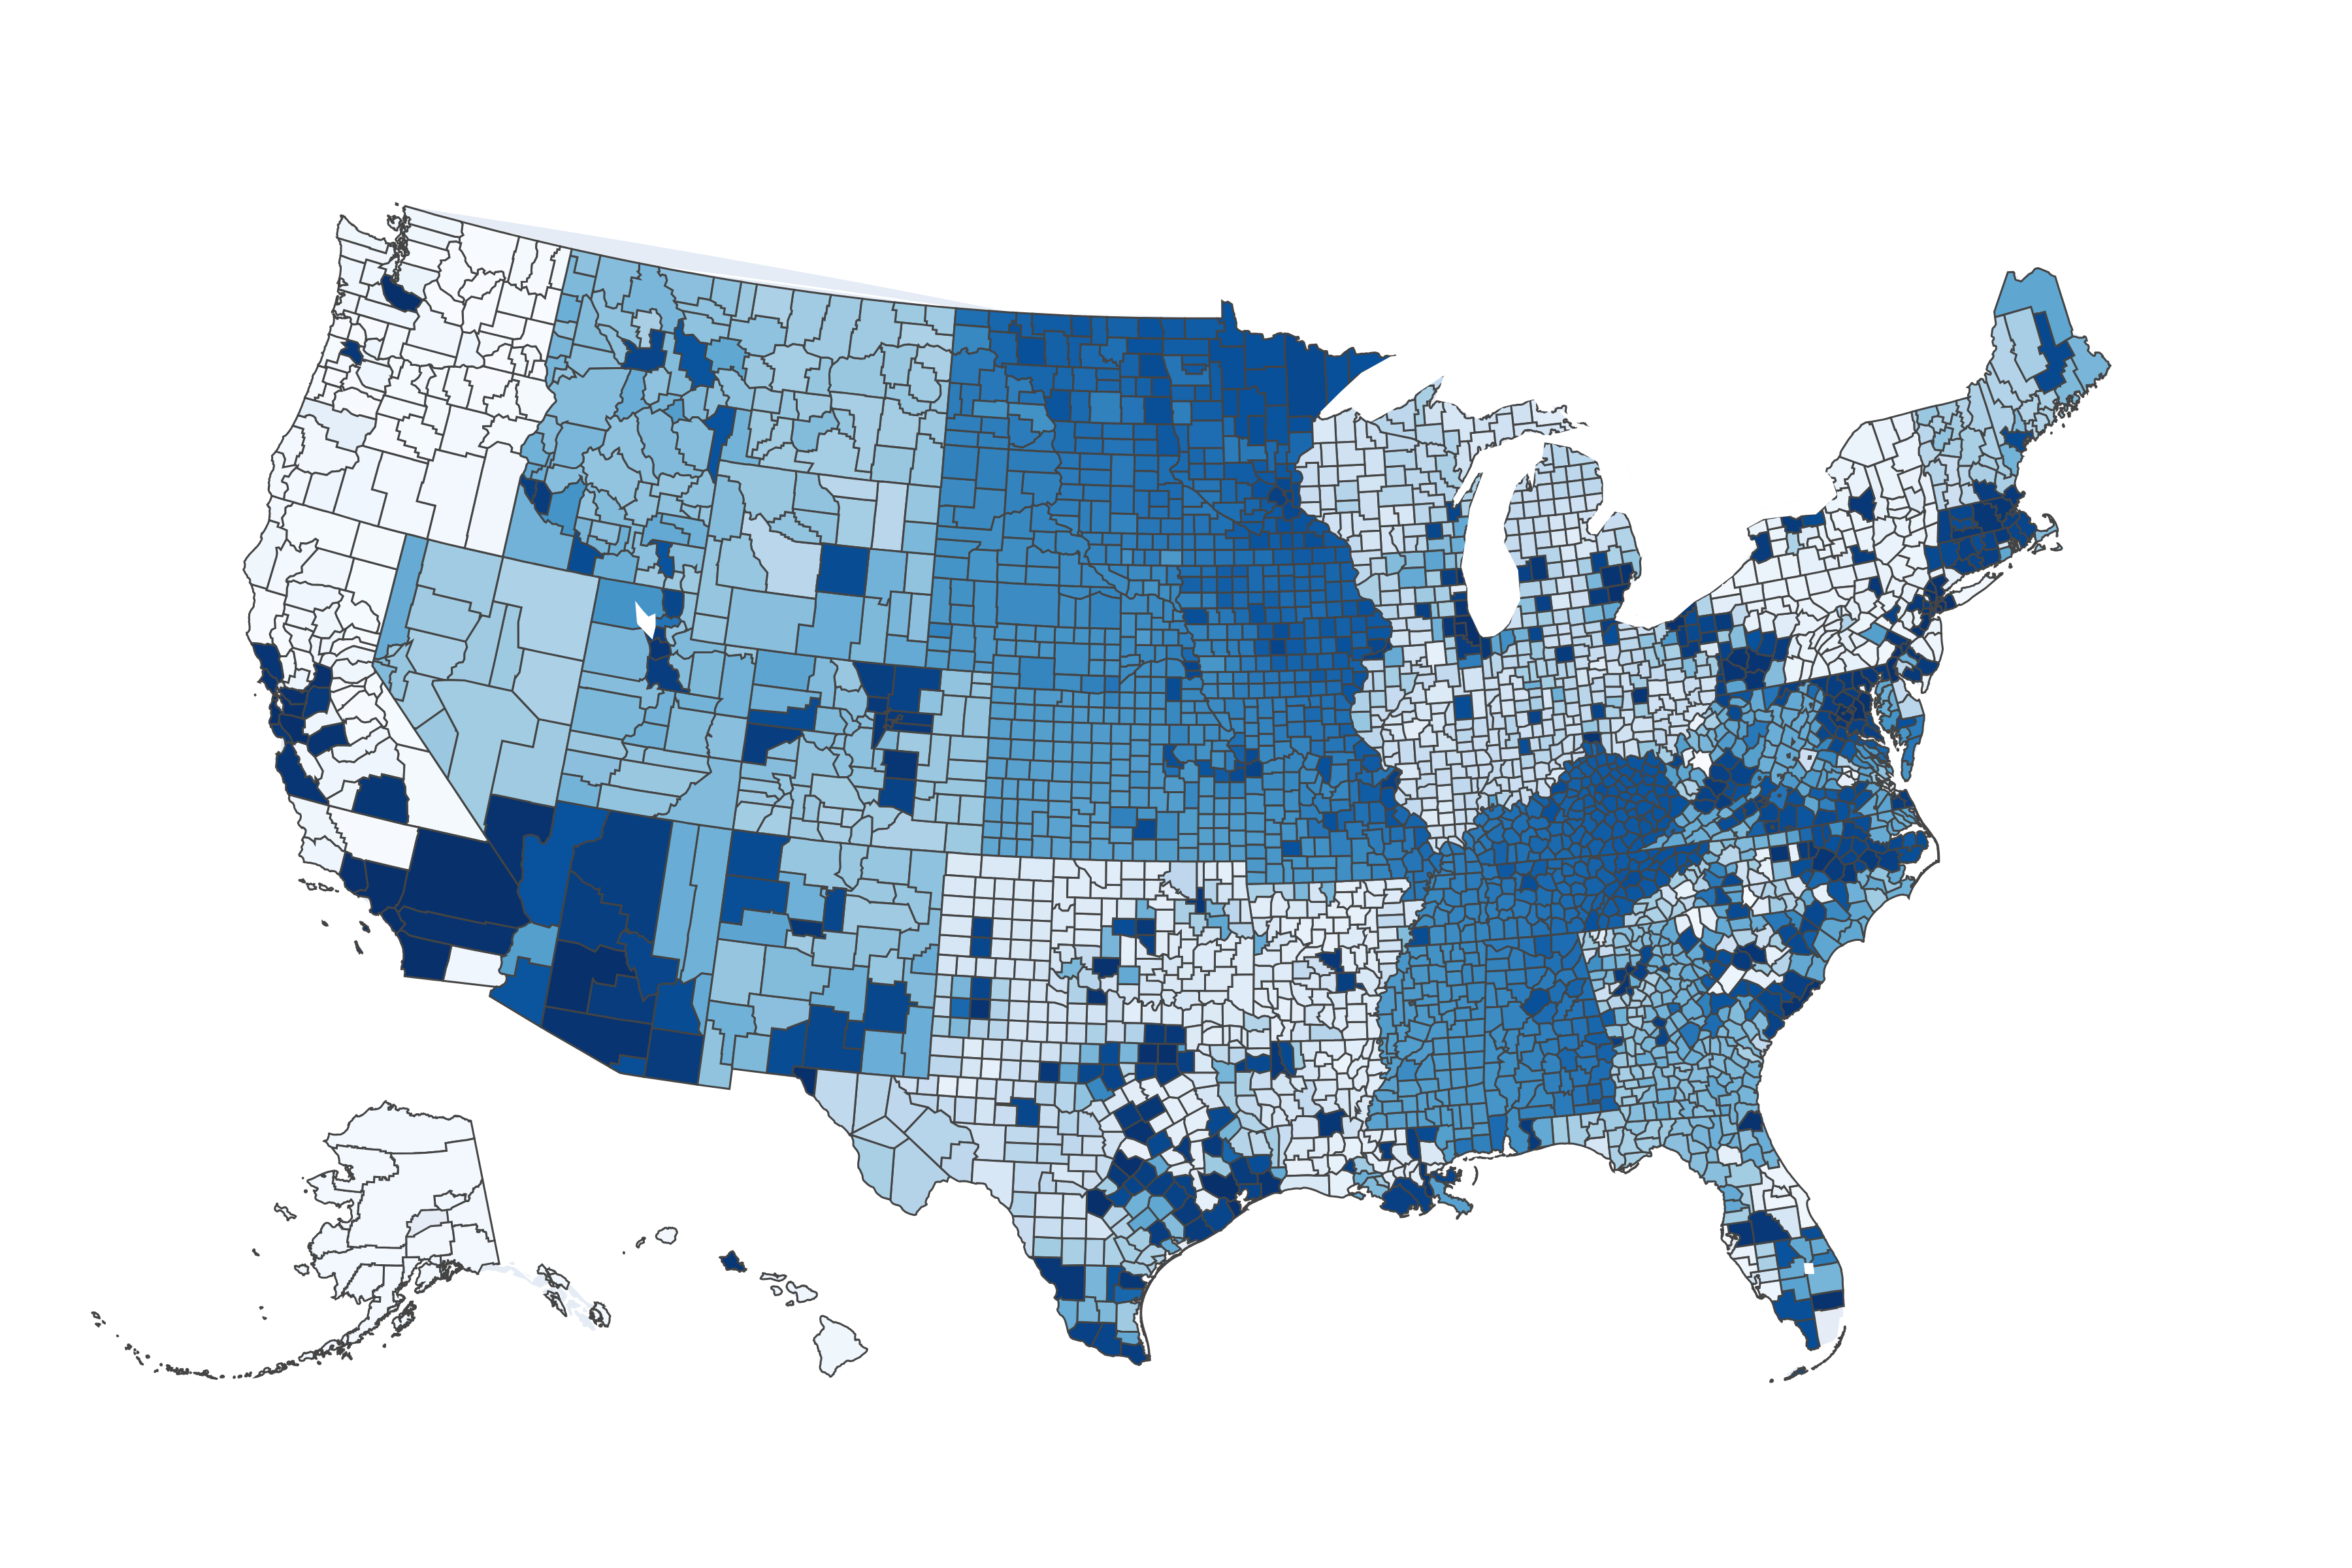
\includegraphics[width=\textwidth]{figures/maps/immigration_shock_1980.png}
        \caption*{\small 1975-1980}
    \end{subfigure}
    \hfill
    \begin{subfigure}[b]{\mapwidth}
        \centering
        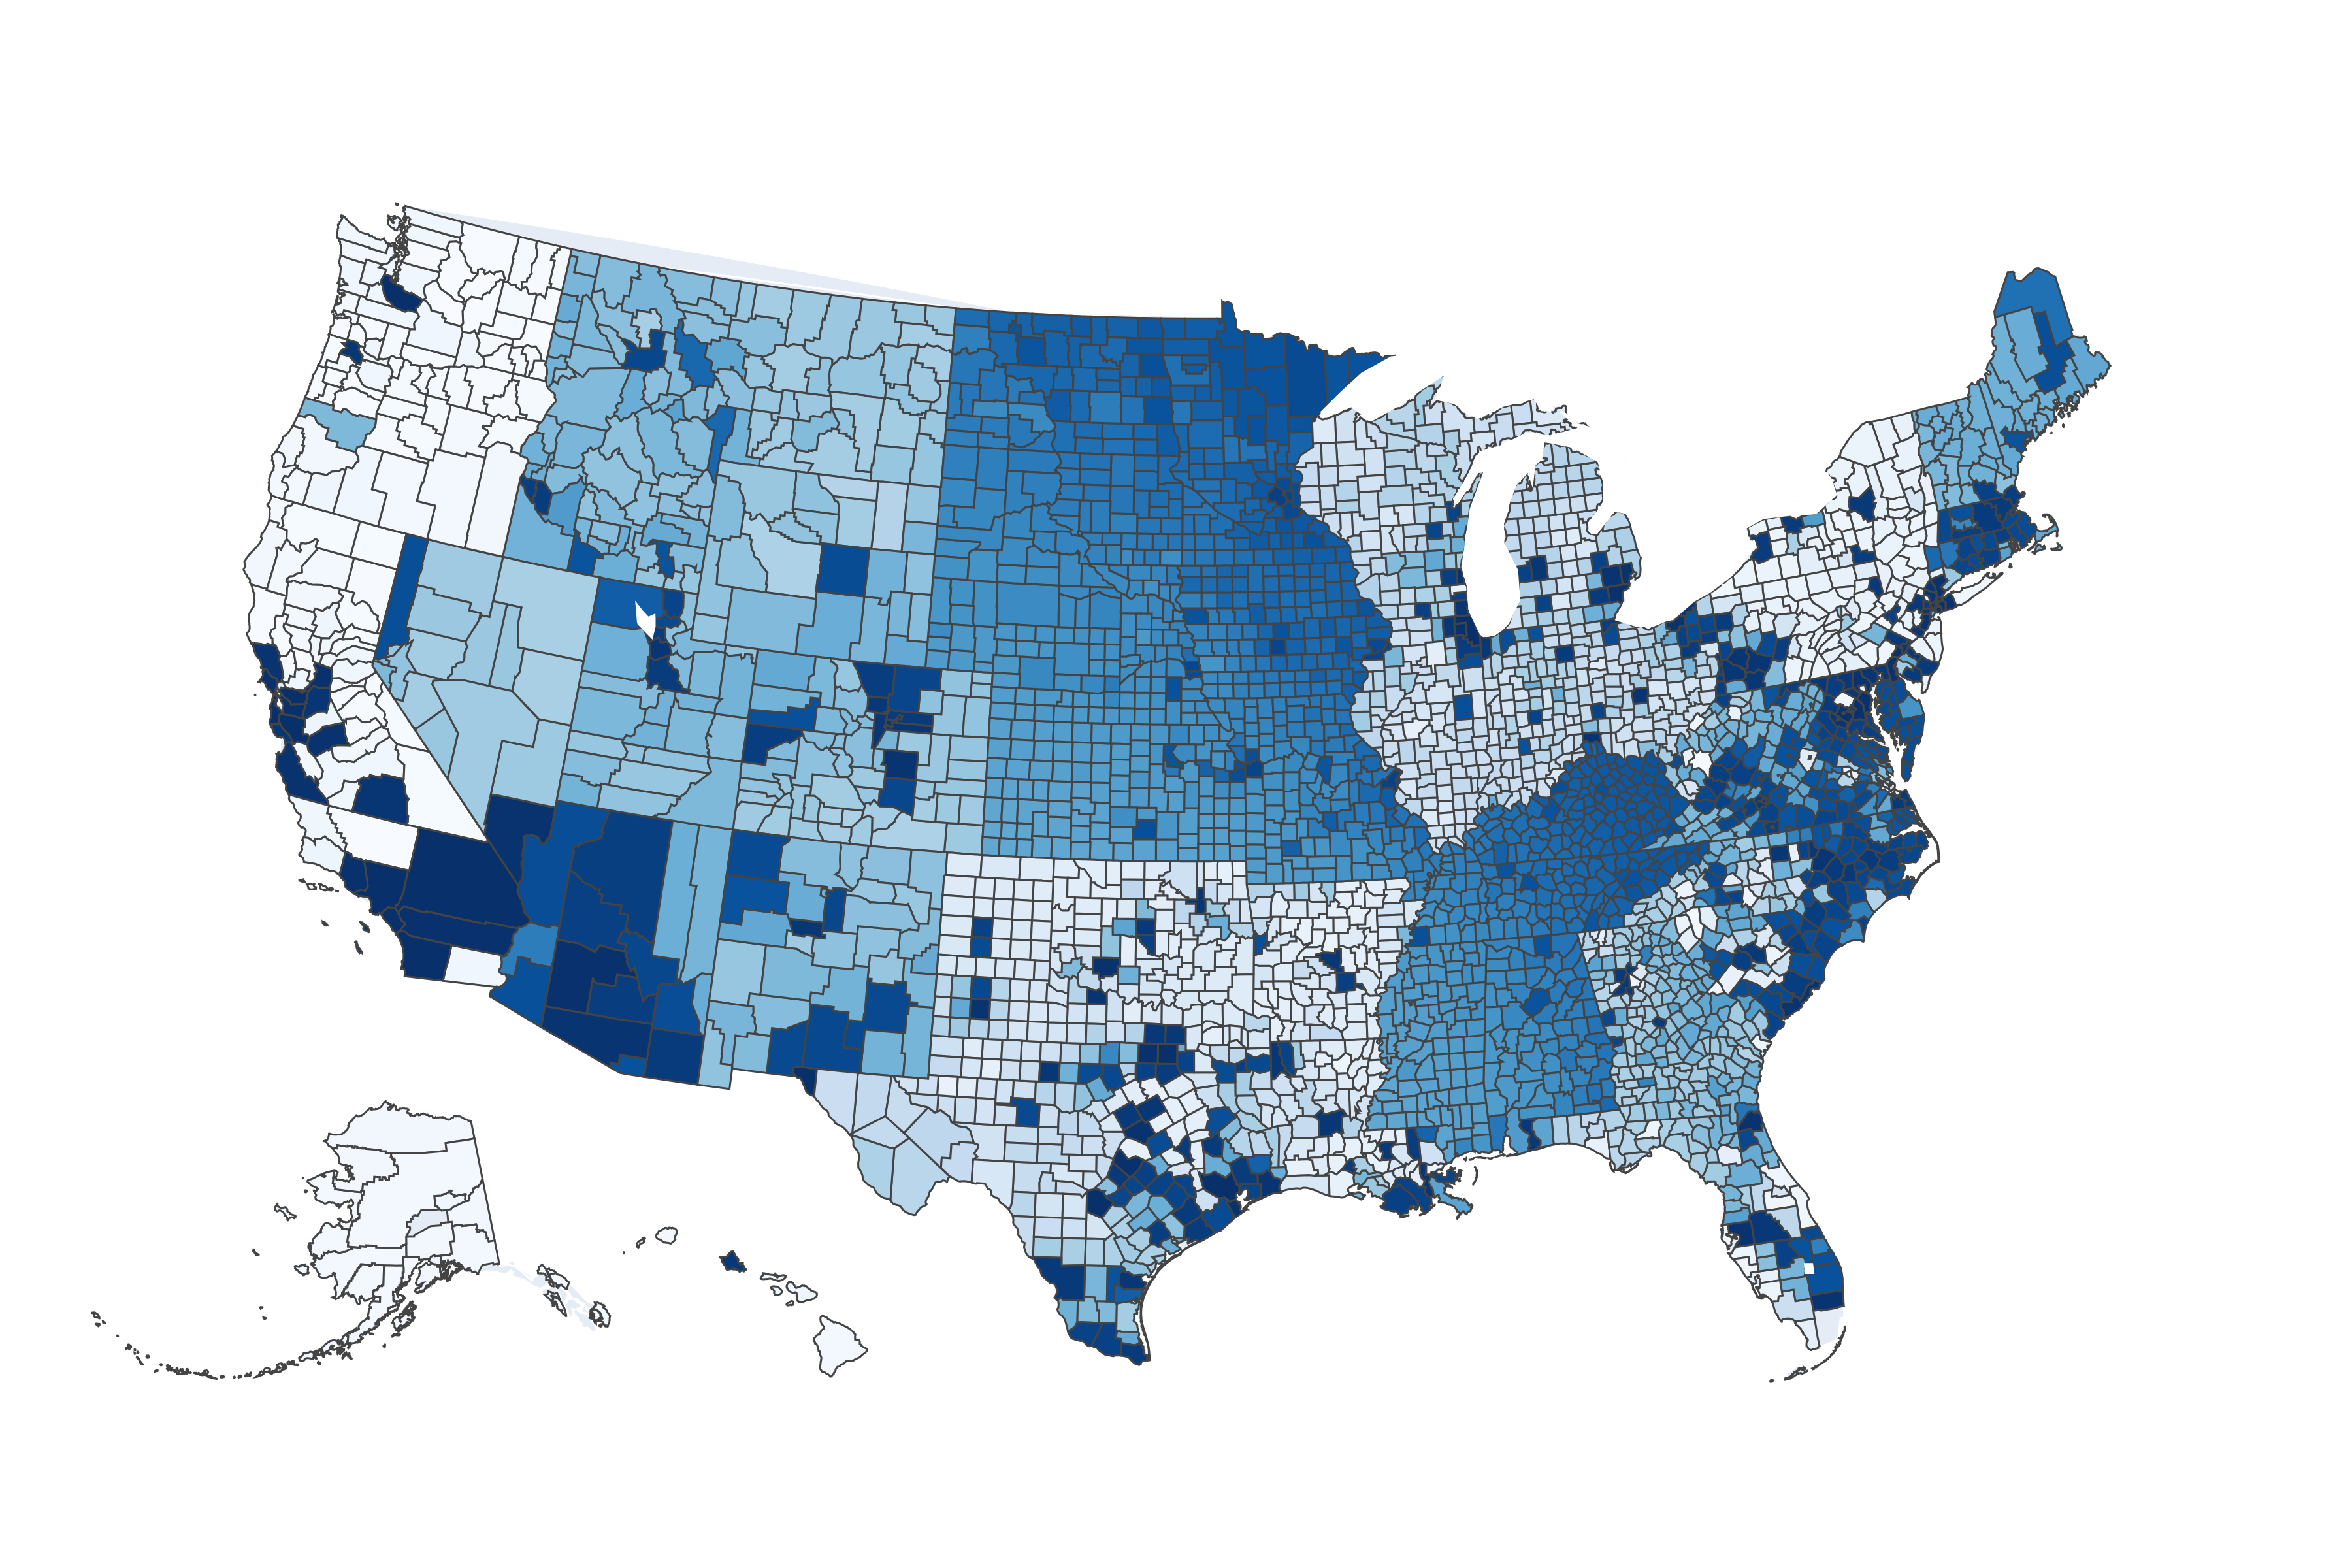
\includegraphics[width=\textwidth]{figures/maps/immigration_shock_1985.png}
        \caption*{\small 1980 - 1985}
    \end{subfigure}
    \hfill
    \begin{subfigure}[b]{\mapwidth}
        \centering
        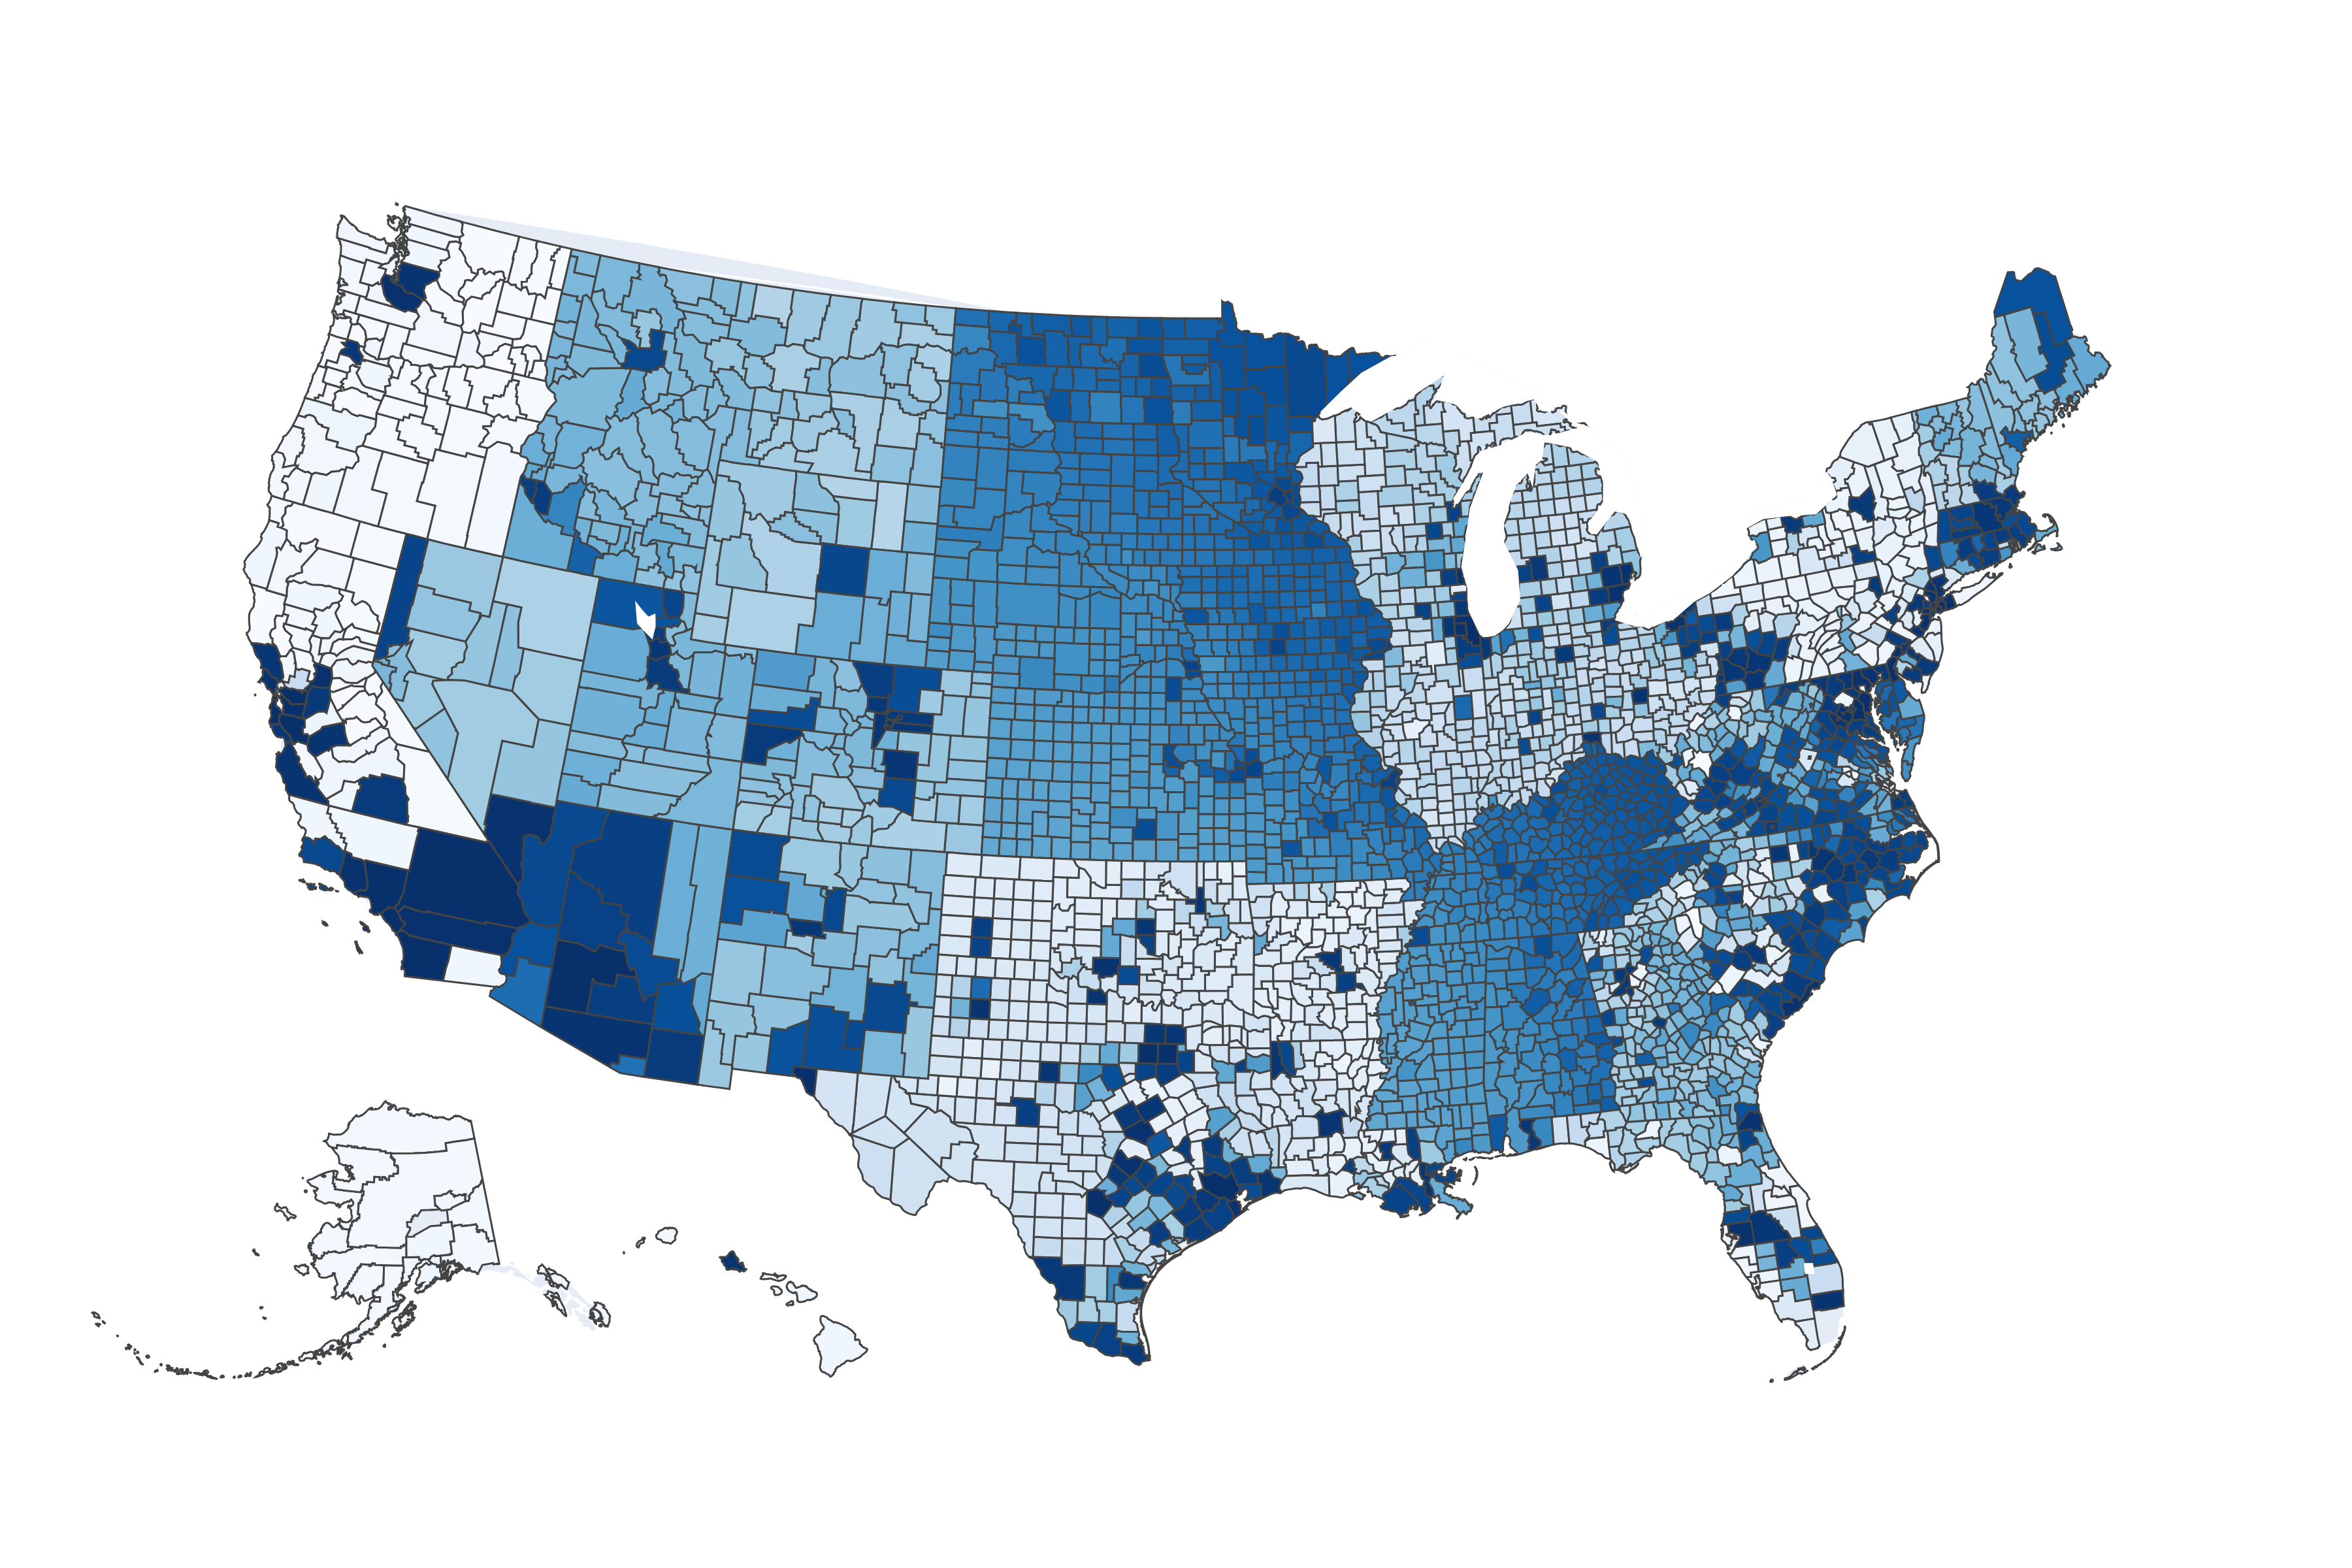
\includegraphics[width=\textwidth]{figures/maps/immigration_shock_1990.png}
        \caption*{\small 1985 - 1990}
    \end{subfigure}
    
    \vspace{0.3em}
    
    % Row 2
    \begin{subfigure}[b]{\mapwidth}
        \centering
        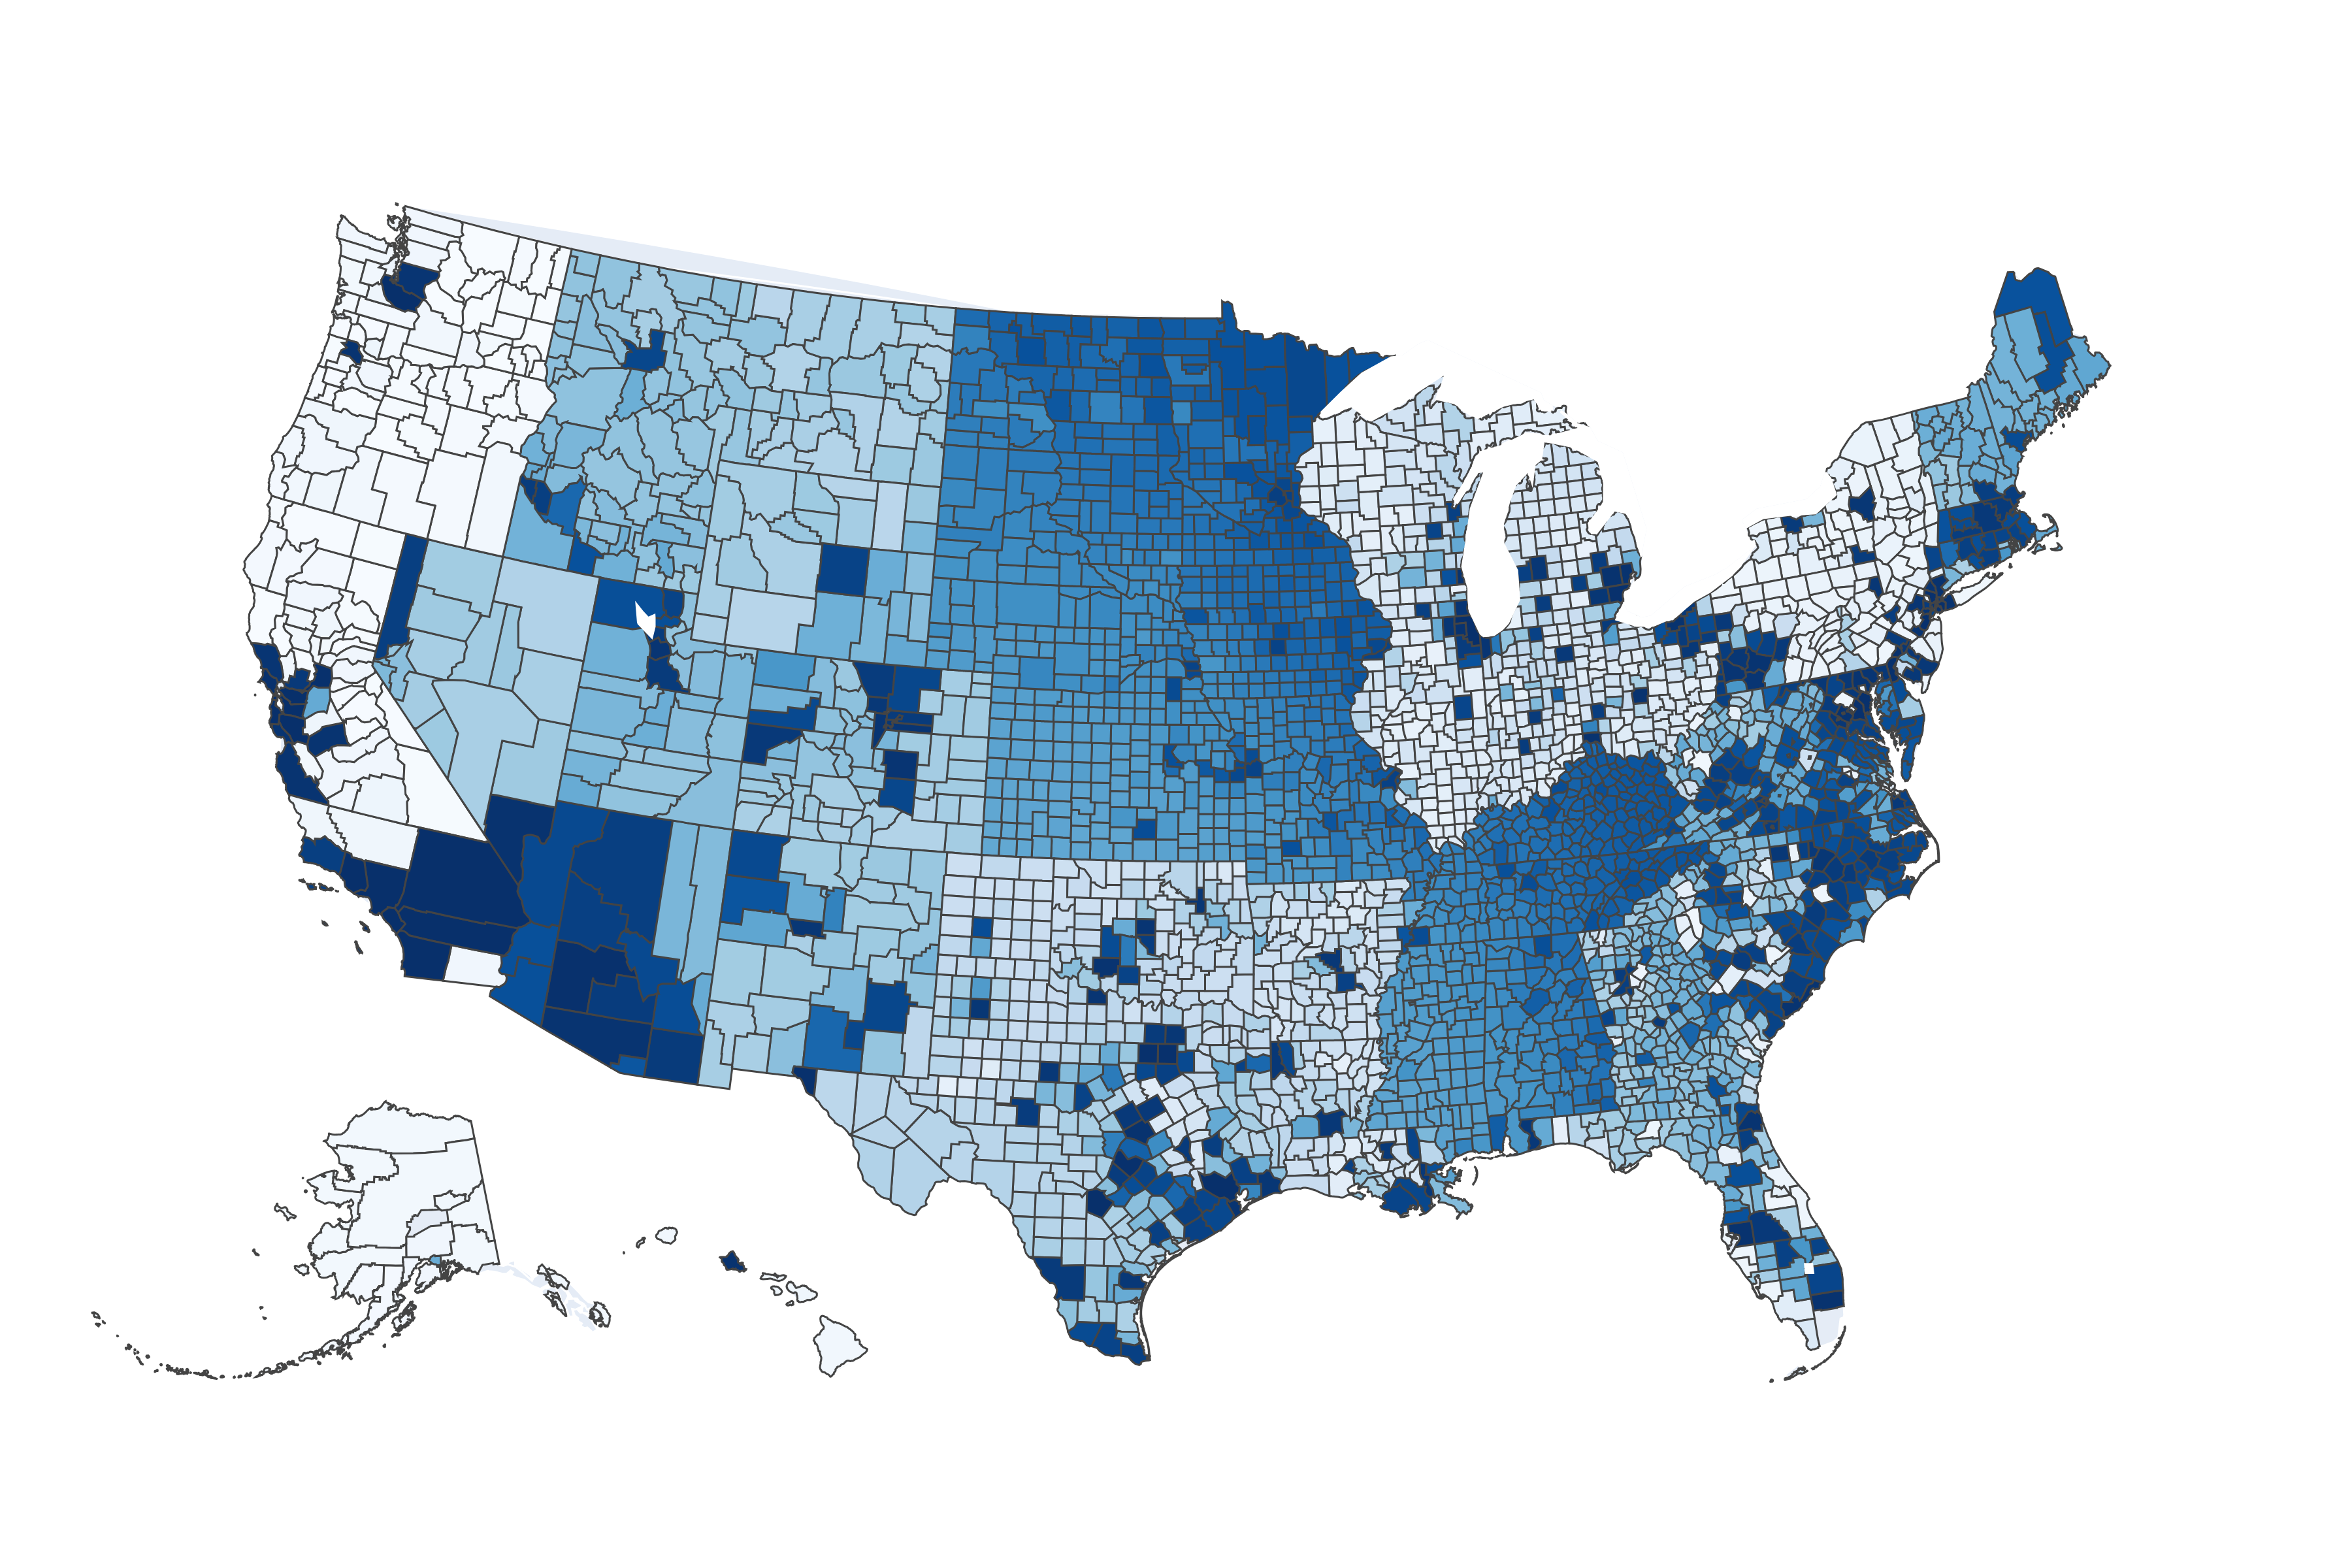
\includegraphics[width=\textwidth]{figures/maps/immigration_shock_1995.png}
        \caption*{\small 1990 - 1995}
    \end{subfigure}
    \hfill
    \begin{subfigure}[b]{\mapwidth}
        \centering
        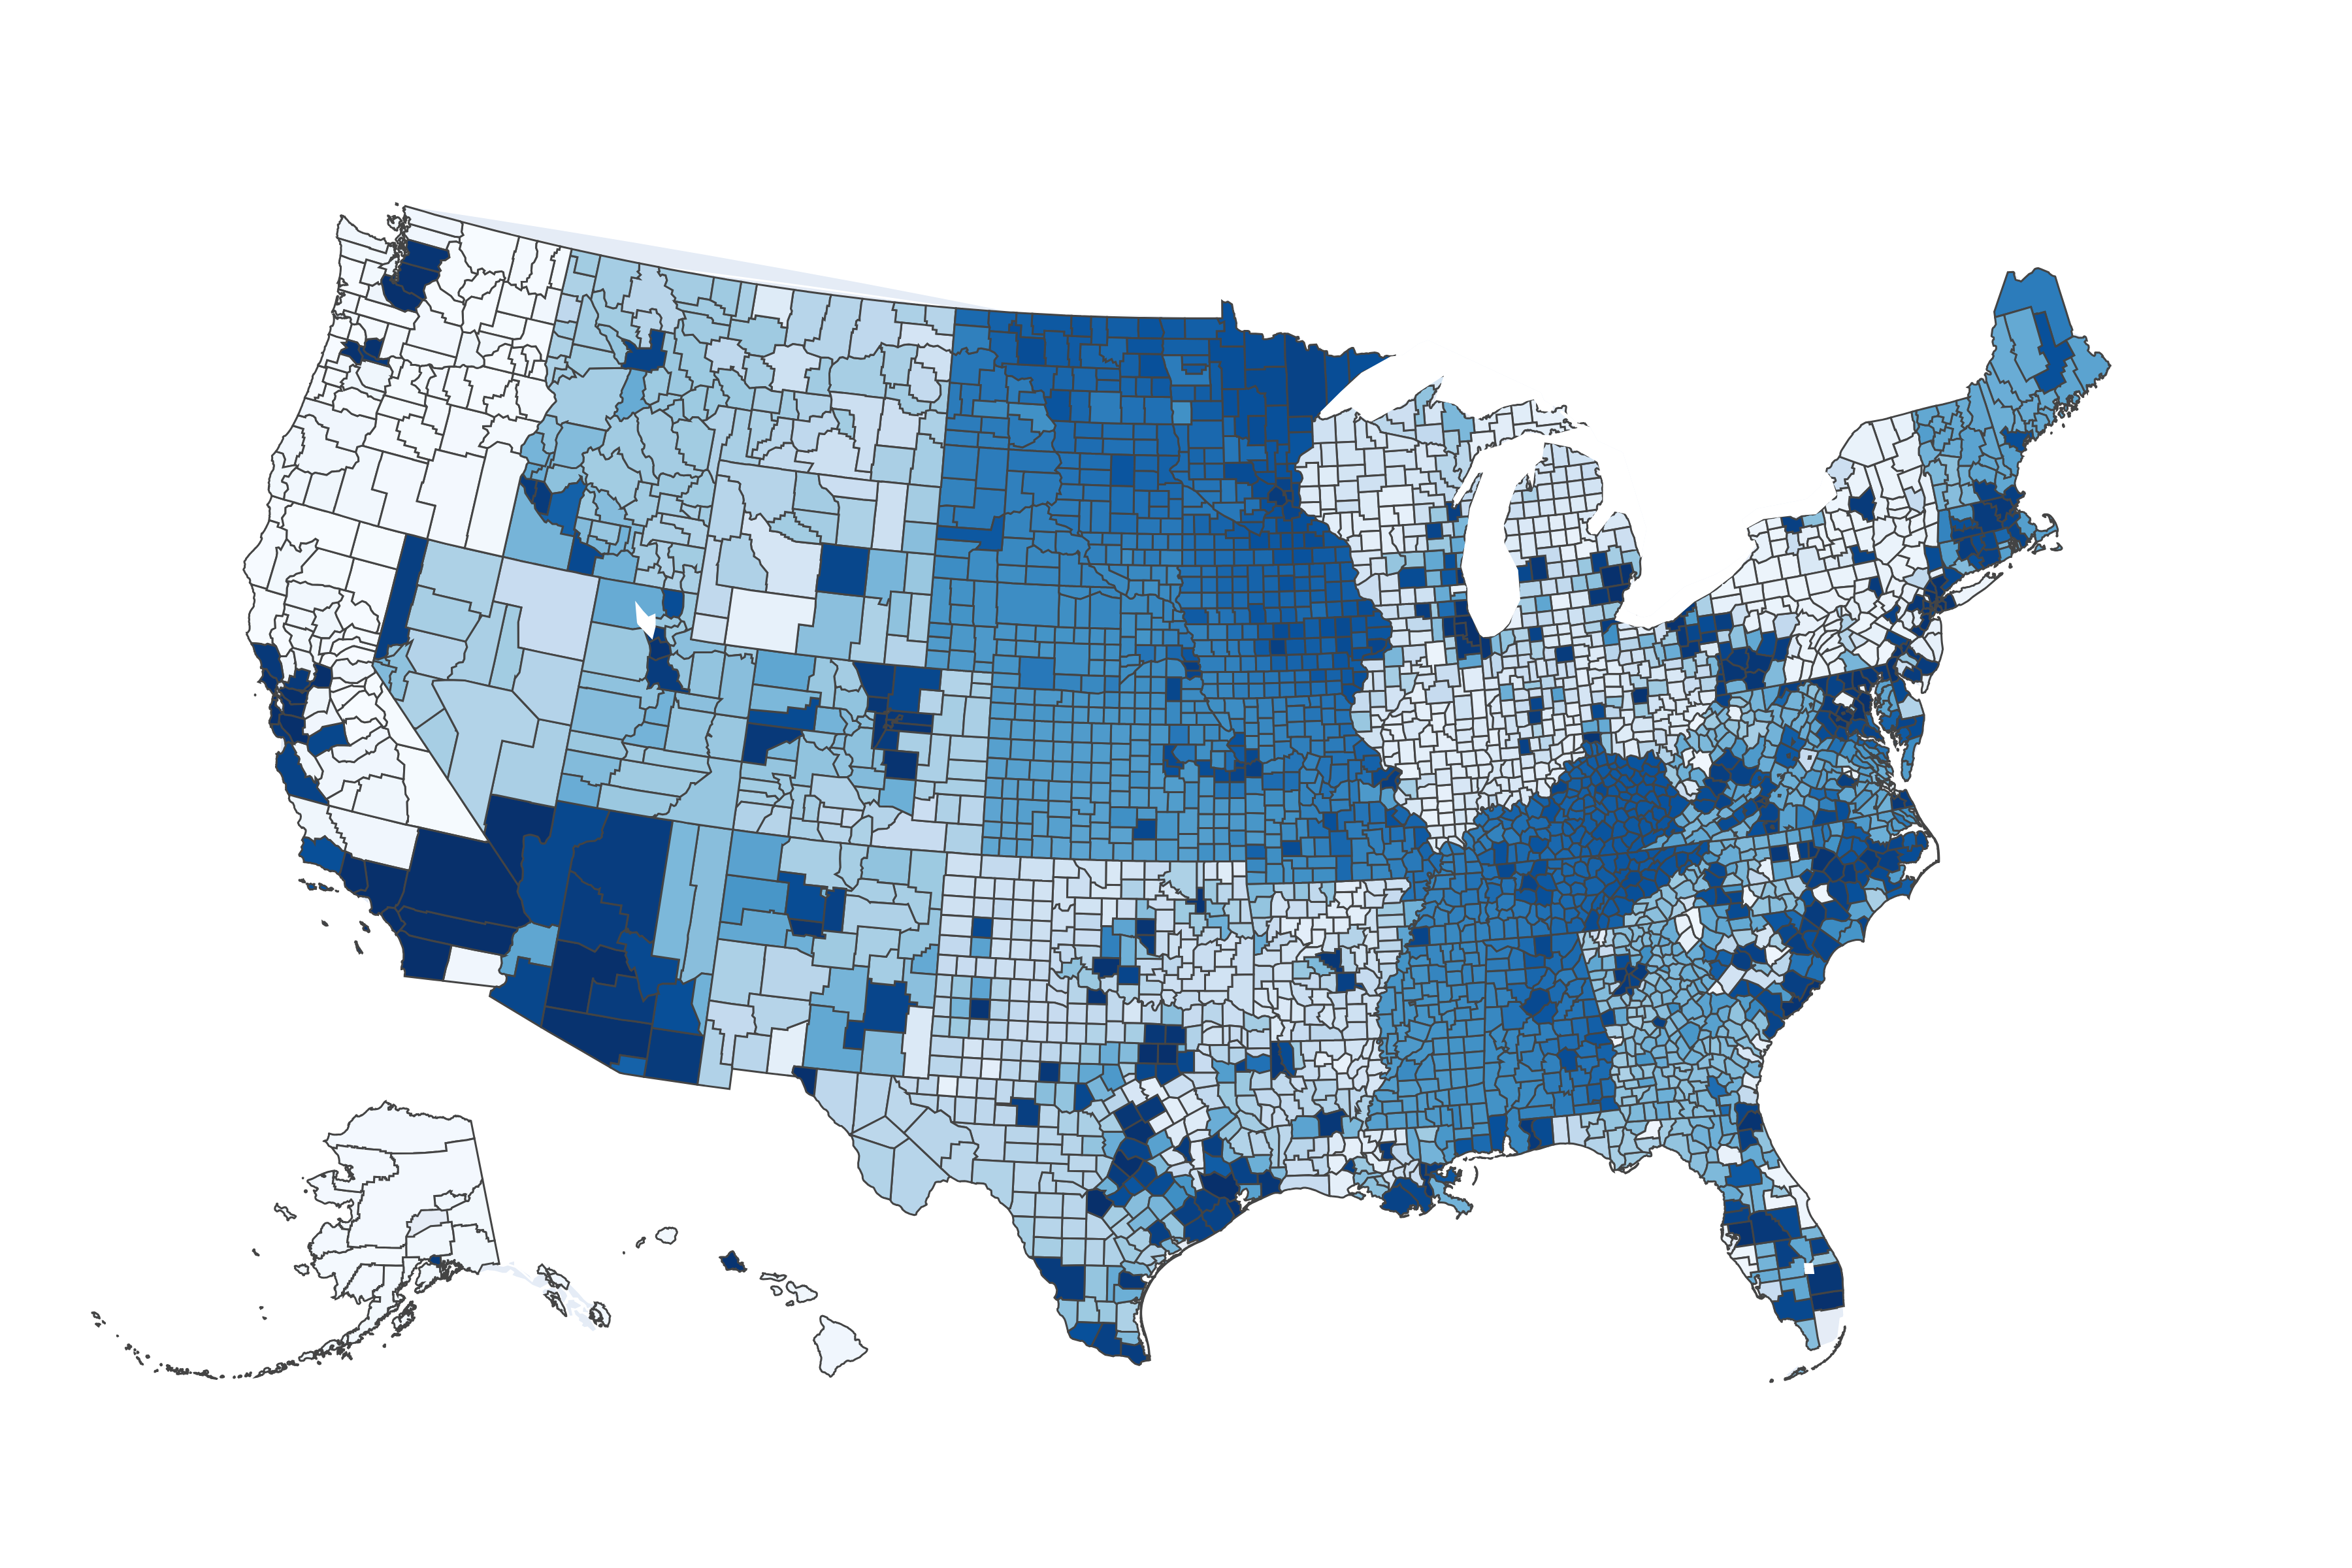
\includegraphics[width=\textwidth]{figures/maps/immigration_shock_2000.png}
        \caption*{\small 1995 - 2000}
    \end{subfigure}
    \hfill
    \begin{subfigure}[b]{\mapwidth}
        \centering
        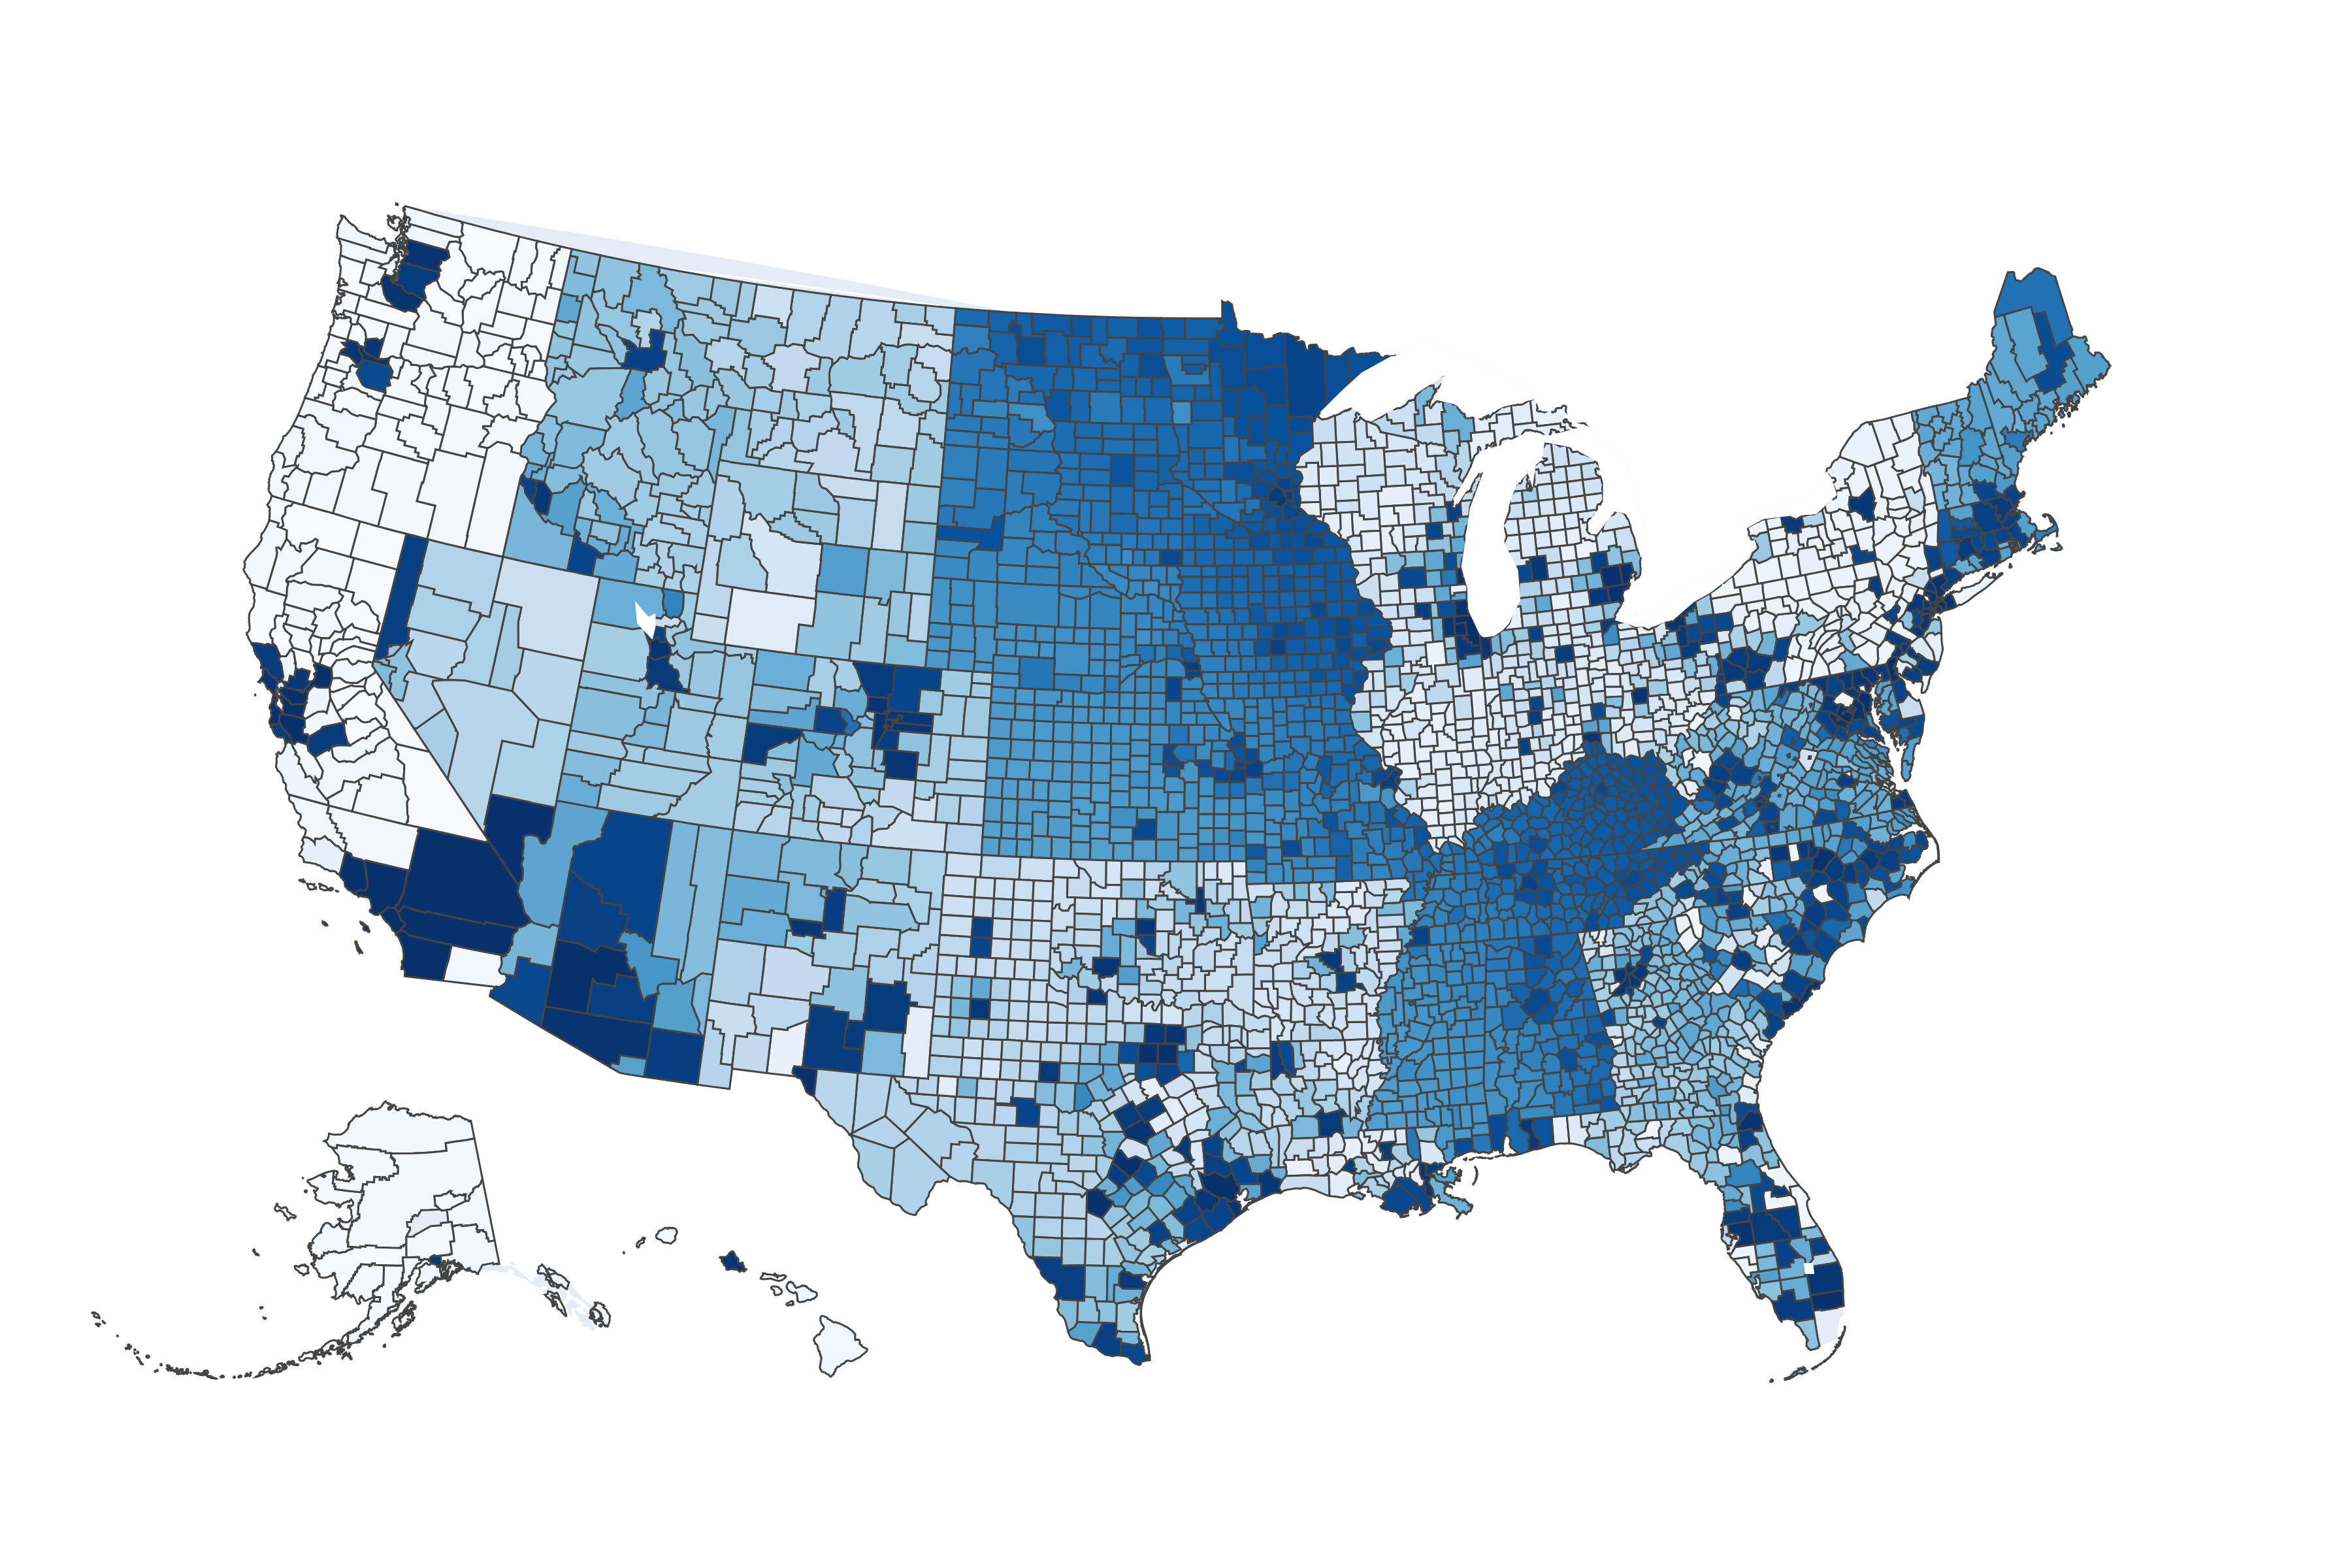
\includegraphics[width=\textwidth]{figures/maps/immigration_shock_2005.png}
        \caption*{\small 2000 - 2005}
    \end{subfigure}
    
    \vspace{0.3em}
    
    % Row 3 (single map, centered)
    \begin{subfigure}[b]{\mapwidth}
        \centering
        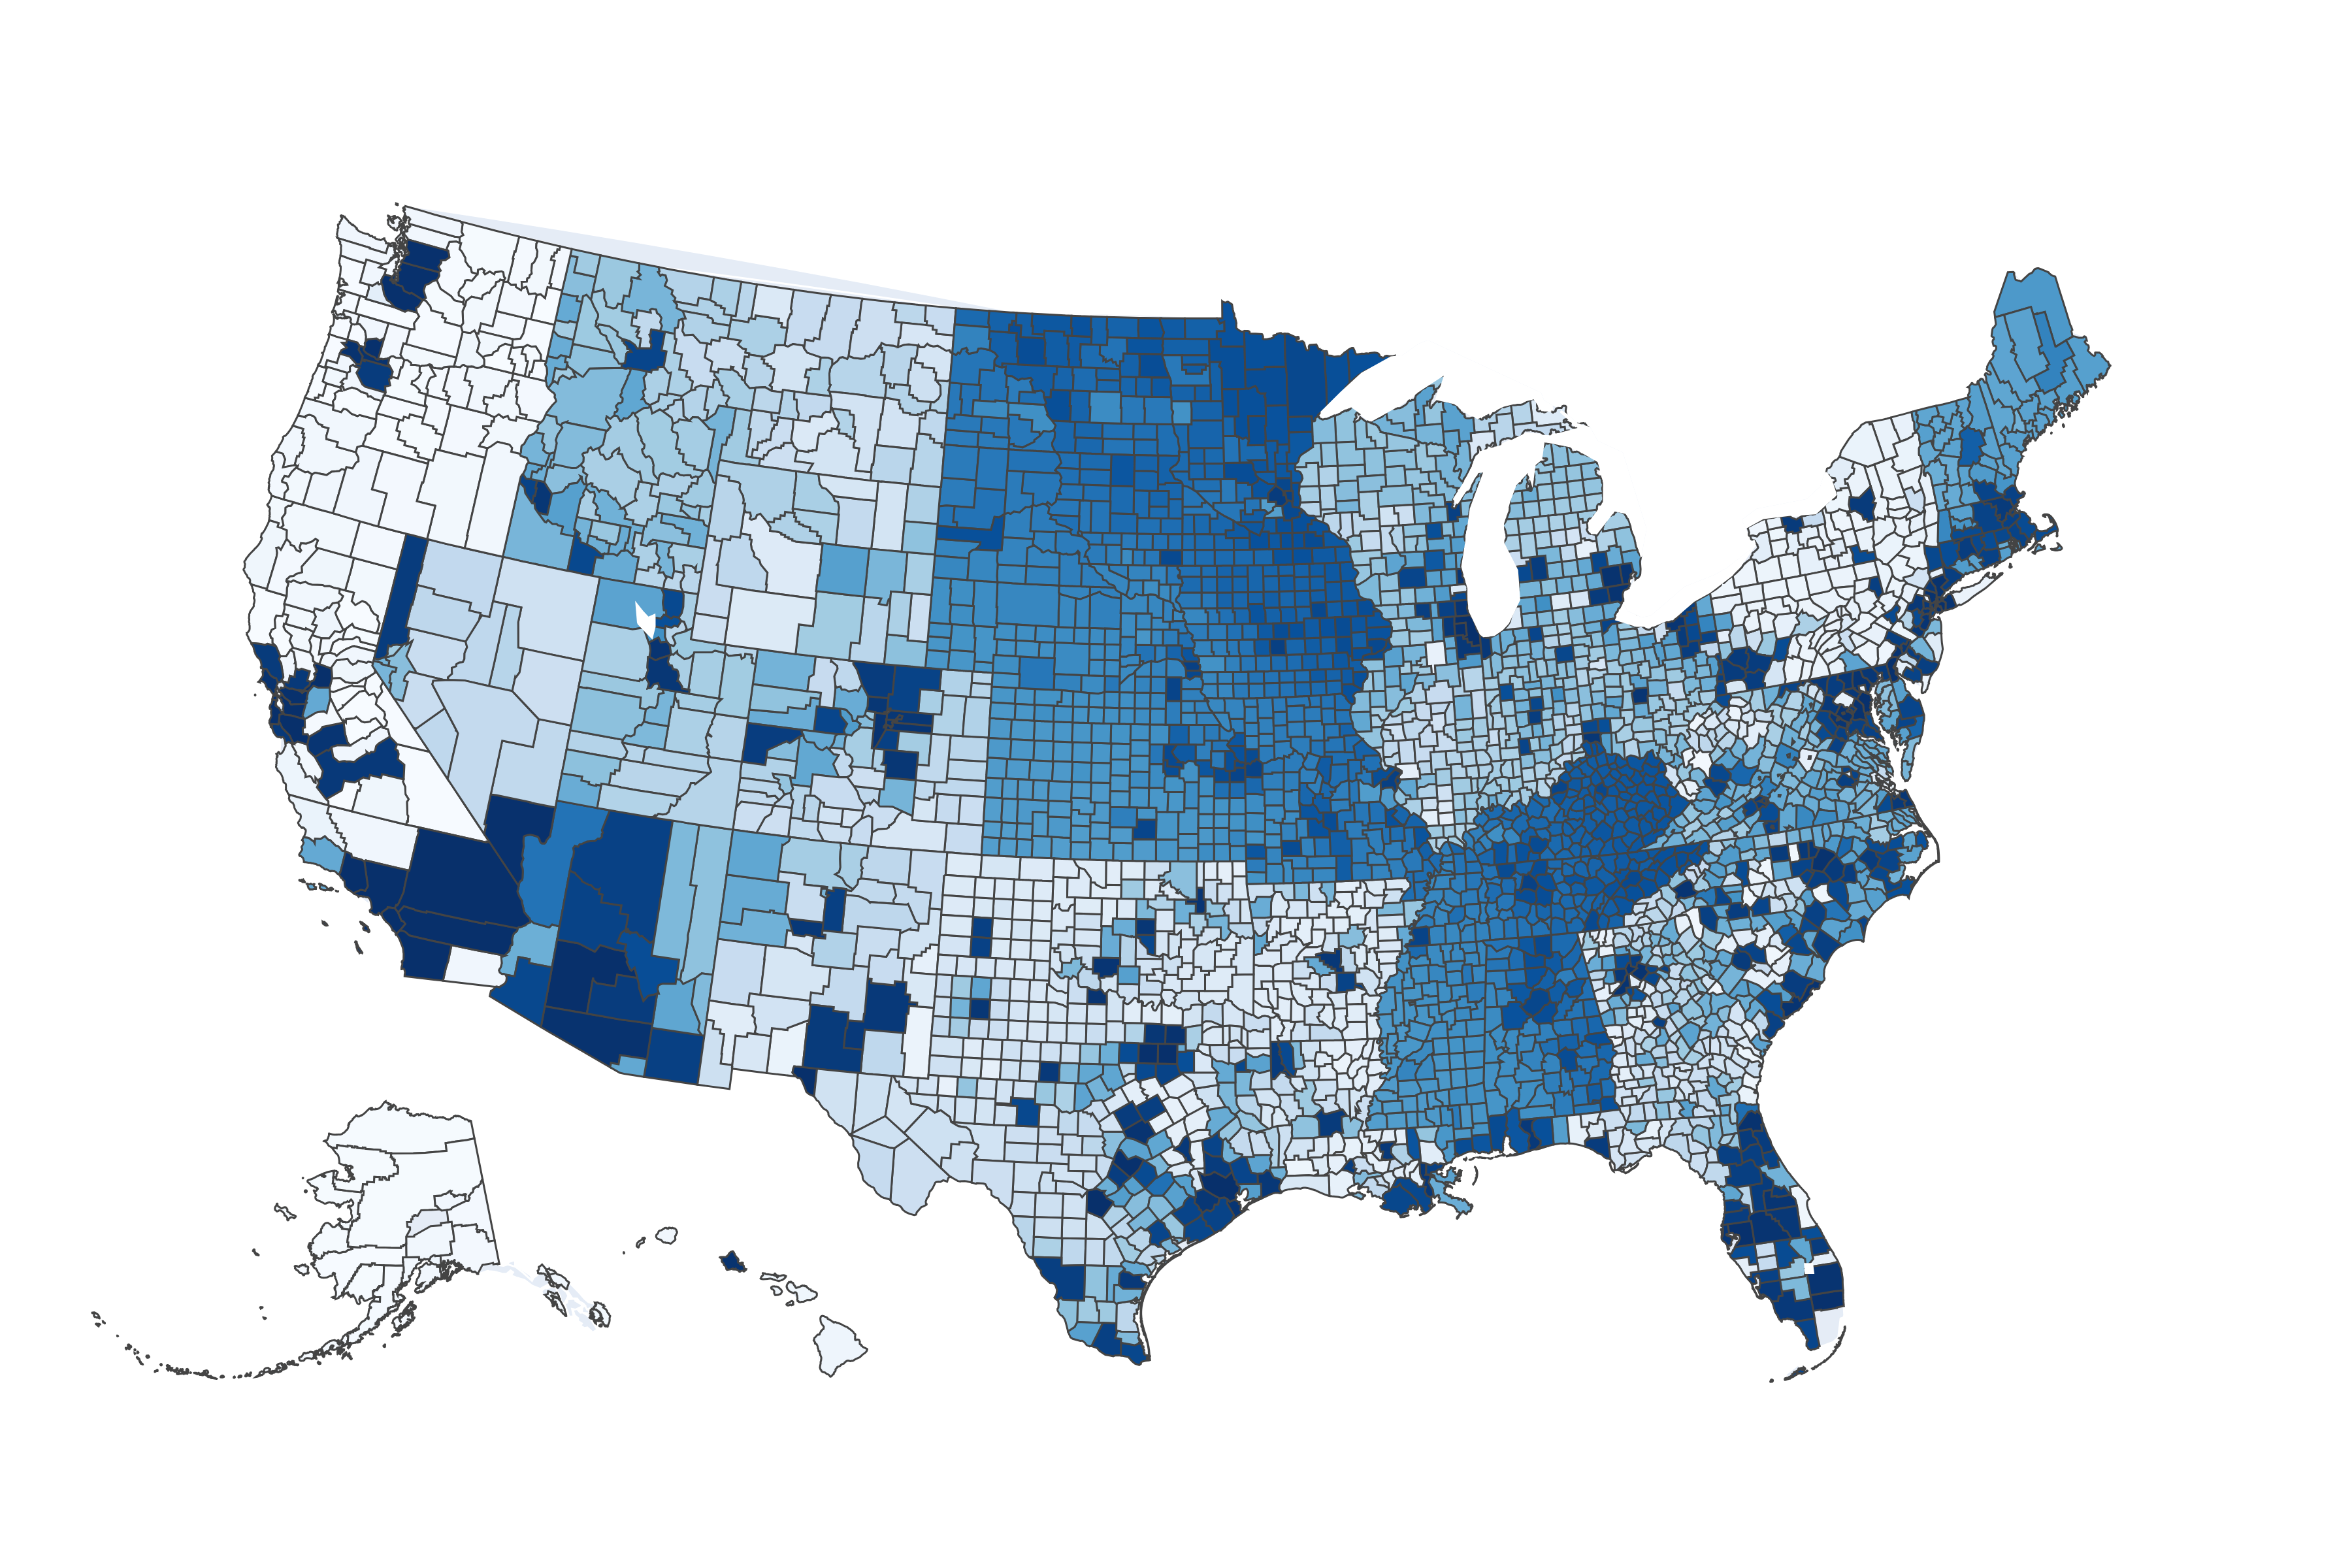
\includegraphics[width=\textwidth]{figures/maps/immigration_shock_2010.png}
        \caption*{\small 2005 - 2010}
    \end{subfigure}
    
    \caption{Immigration Shocks (Instruments) for 5-year periods. The map's color depicts data broken into 200 quantiles with darker colors representing larger values.}
    \label{fig:immigration_map}
\end{figure}
\begin{table}[htbp]\centering
\def\sym#1{\ifmmode^{#1}\else\(^{#1}\)\fi}
\caption{Immigration Data \label{tab:immigration}}
\begin{tabular}{l*{1}{ccccc}}
\toprule
                    &           N&        Mean&         Min&         Max&          SD\\
\midrule
Immigration Instrument&       21987&       0.000&      -7.807&     377.218&       4.991\\
5-year Non-European Immigration&       21987&       1.418&      -0.000&     777.956&      12.214\\
5-year Immigration  &       21987&       1.614&       0.000&     825.411&      13.332\\
\bottomrule
\multicolumn{6}{l}{\footnotesize All observations are at the county 5-year level. Immigration numbers are reported in 1000s.}\\
\end{tabular}
\end{table}

% \begin{table}[htbp]\centering
\def\sym#1{\ifmmode^{#1}\else\(^{#1}\)\fi}
\caption{Business Dynamics Data \label{tab:bds}}
\begin{tabular}{l*{1}{ccccc}}
\toprule
                    &           N&        Mean&         Min&         Max&          SD\\
\midrule
Firm Count          &           0&           .&           .&           .&           .\\
Establishment Count &     105,314&     1,802.5&           0&   216,895.0&     6,070.3\\
Employment          &     105,314&    30,426.5&           0& 3,781,728.0&   115,528.3\\
Establishment Births&           0&           .&           .&           .&           .\\
Establishment Entry Rate&     103,836&        11.7&           0&       120.0&         4.0\\
Establishment Exits &           0&           .&           .&           .&           .\\
Establishment Exit Rate&     103,692&        10.6&           0&        86.7&         3.2\\
Job Creation        &           0&           .&           .&           .&           .\\
Job Creation (New Estabs.)&           0&           .&           .&           .&           .\\
Job Creation (Continuers)&           0&           .&           .&           .&           .\\
Job Destruction     &           0&           .&           .&           .&           .\\
Job Destruction (Dead Estabs.)&           0&           .&           .&           .&           .\\
Job Destruction (Continuers)&           0&           .&           .&           .&           .\\
Net Job Creation    &           0&           .&           .&           .&           .\\
\bottomrule
\multicolumn{6}{l}{\footnotesize All observations are at the county year level. Data is from 1978 to 2010.}\\
\end{tabular}
\end{table}

\begin{table}[htbp]\centering\caption{Survey Data by Ownership Type \label{tab:sbo}}\begin{tabular}{l*{4}{c}}\toprule & (1) & (2) & (3) & (4) \\
& All & Fully American & Fully Immigrant & Mixed \\ \midrule \midrule
Firm Age            &       10.40&       11.17&        7.89&       10.19\\
                    &      (9.31)&      (9.45)&      (8.08)&      (9.10)\\
Employment          &        2.25&        3.22&        2.09&        5.29\\
                    &     (43.87)&     (44.96)&     (20.30)&     (36.68)\\
Payroll             &       73.54&      109.56&       58.76&      205.17\\
                    &  (1,448.12)&  (1,668.95)&    (743.13)&  (2,319.76)\\
Receipts            &      414.80&      594.50&      377.23&      967.57\\
                    & (10,917.16)& (11,016.27)&  (6,609.19)& (15,618.69)\\
Family Business     &        0.28&        0.28&        0.20&        0.65\\
                    &      (0.45)&      (0.45)&      (0.40)&      (0.48)\\
Couple-Owned        &        0.26&        0.26&        0.23&        0.59\\
                    &      (0.44)&      (0.44)&      (0.42)&      (0.49)\\
Home Based Business &        0.54&        0.55&        0.41&        0.45\\
                    &      (0.50)&      (0.50)&      (0.49)&      (0.50)\\
Has Full Time Employees&        0.25&        0.27&        0.28&        0.39\\
                    &      (0.43)&      (0.44)&      (0.45)&      (0.49)\\
\midrule
Observations &   26,392,237 &   11,706,283 &    1,769,548 &      424,057 \\\bottomrule\end{tabular}\par\smallskip\raggedright\footnotesize Notes: All observations are at the firm/business level. Cell values report weighted means with weighted standard deviations in parentheses. Observation counts reflect weighted number of firms.\end{table}




\begin{figure}
    \centering
    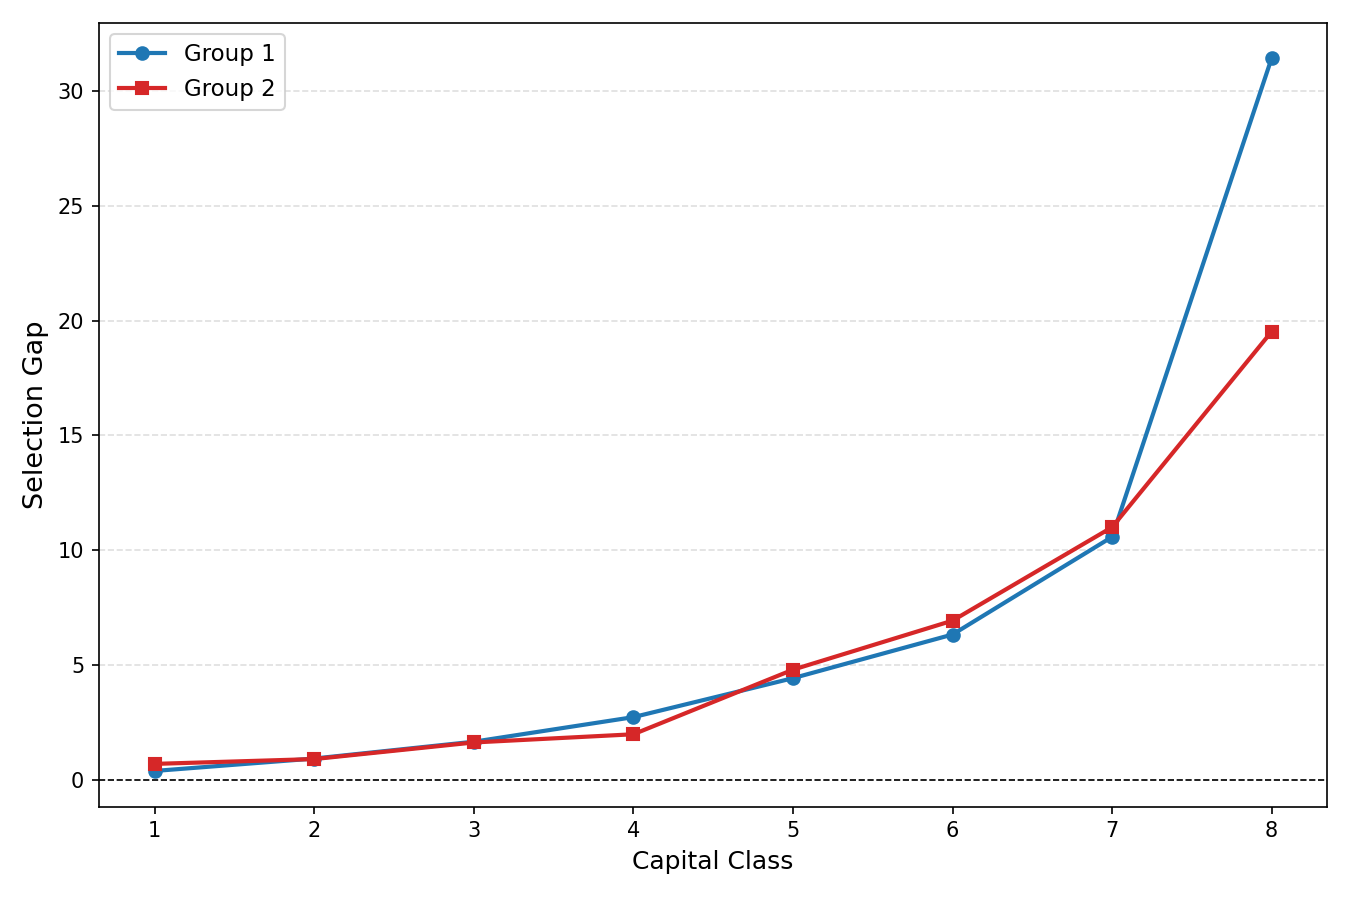
\includegraphics[width=\linewidth]{figures/gap_simulation.png}
    \caption{Selection Gap Using Simulated Data}
    \label{fig:gap_simulation}
\end{figure}

\begin{table}
    \centering
\begin{tabular}{lccc}
\multicolumn{4}{c}{\large \textbf{Firms in Top Capital Bucket}} \\
\toprule \toprule
 & \multicolumn{2}{c}{\textbf{Firm Size}} & \textbf{Selection Gap} \\
\cmidrule(lr){2-3}  & New Firms & Young Firms &  \\
\midrule 
Native & 6.41 & 11.98 & 5.57 \\
Immigrant & 7.30 & 11.14 & 3.83 \\
\midrule
Difference & -0.89 & 0.84 & 1.74 \\
\bottomrule \bottomrule
\multicolumn{4}{l}{\small\textit{Note:} New firms are defined as those of ages 0 and 1 while} \\
\multicolumn{4}{l}{\small young firms are of ages 2 and 3 years.} 
\end{tabular}
 \caption{Selection Gap From 2007 SBO Data}
    \label{tab:selection_gap}\end{table}


\begin{figure}
    \centering
    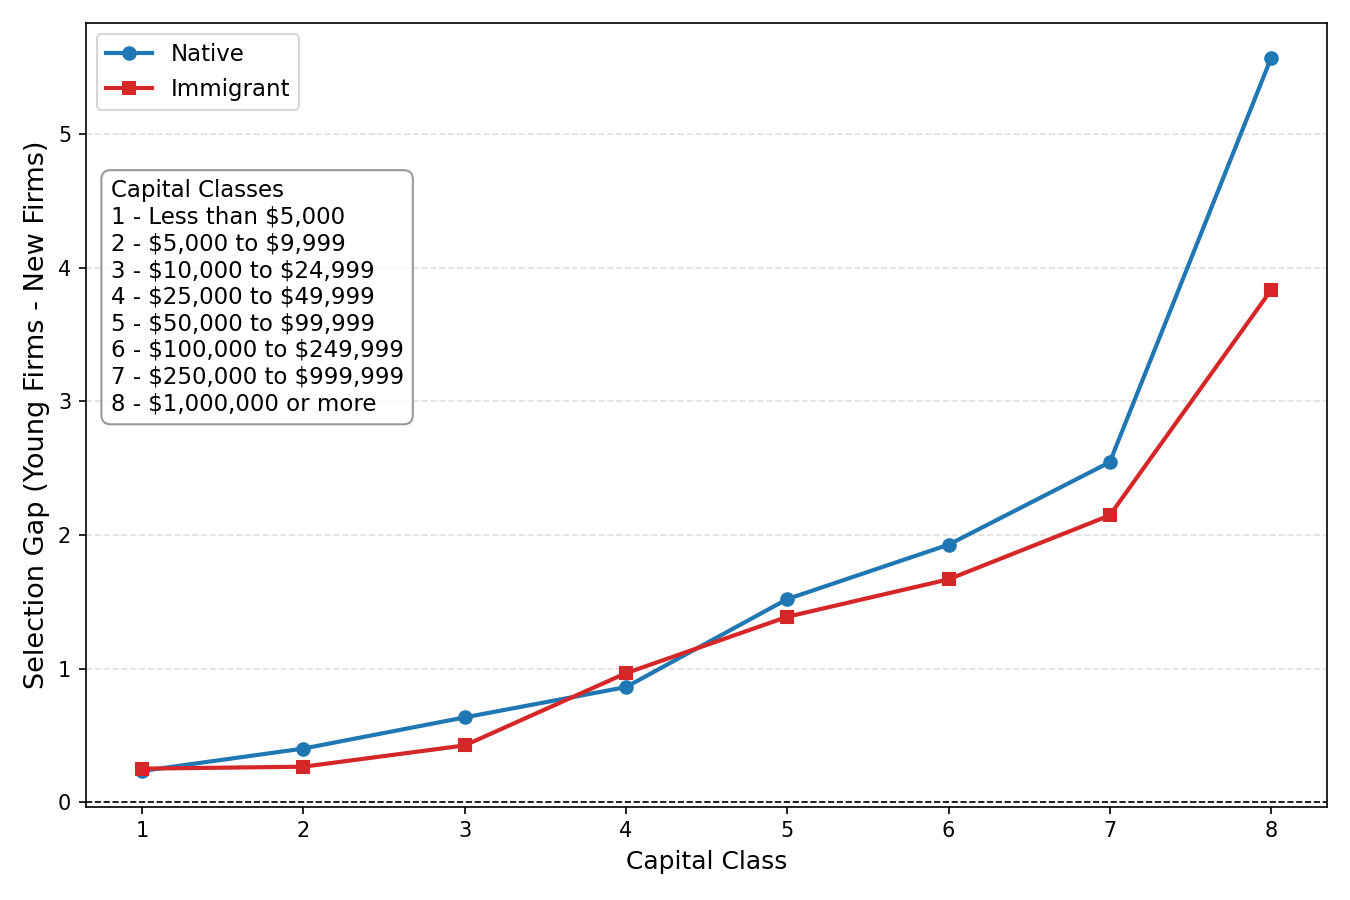
\includegraphics[width=\linewidth]{figures/selection_gap.png}
    \caption{Selection Gap using 2007 SBO Data}
    \label{fig:gap_data}
\end{figure}



\begin{table}[htbp]
\centering
\caption{IV First Stage}
\label{tab:firststage}
\begin{tabular}{l*{3}{c}}
\toprule
& \multicolumn{3}{c}{Non-European Migration} \\
\cmidrule(lr){2-4}
& (1) & (2) & (3) \\
\midrule
Immigration Shock&       2.090\sym{***}&       2.094\sym{***}&       2.096\sym{***}\\
            &     (0.053)         &     (0.056)         &     (0.037)         \\
\midrule
N           &       21854         &       21847         &       21854         \\
R$^2$       &       0.818         &       0.823         &       0.793         \\
P-value     &       0.000         &       0.000         &       0.000         \\
Geography FE&       State         &       State         &      County         \\
Time FE     &         Yes         &         Yes         &         Yes         \\
State-Time FE&          No         &         Yes         &          No         \\
\bottomrule
\multicolumn{4}{@{}l@{}}{\footnotesize \textit{Notes:} * p$<$0.10, ** p$<$0.05, *** p$<$0.01.}
\\
\multicolumn{4}{@{}l@{}}{\footnotesize Standard errors clustered at the state level.}
\\
\end{tabular}
\end{table}


\begin{table}[htbp] \centering
\caption{Effects on Business Dynamics}
\label{tab:main}
\newsavebox{\boxmain} \newlength{\tablemain}
\savebox{\boxmain}{\begin{tabular}{lcccc} \toprule
& (1) & (2) & (3) & (4)  \\ \cmidrule(lr){2-5}
                    &\multicolumn{1}{c}{Wages}&\multicolumn{1}{c}{Firm Size}&\multicolumn{1}{c}{Entry Rate}&\multicolumn{1}{c}{Exit Rate}\\
\midrule
Log(Immigration)    &       0.080\sym{***}&       0.101\sym{***}&       0.183\sym{***}&       0.117\sym{***}\\
                    &     (0.006)         &     (0.006)         &     (0.051)         &     (0.019)         \\
\midrule
N                   &       12388         &       18492         &       14923         &       14918         \\
F-stat              &       368.2         &       495.7         &       450.7         &       450.3         \\
P-value             &       0.000         &       0.000         &       0.001         &       0.000         \\
\bottomrule \end{tabular} }
\settowidth{\tablemain}{\usebox{\boxmain}}
\usebox{\boxmain} \vspace{0.5em} 
\parbox{\tablemain}{\footnotesize \textit{Notes:} * p$<$0.10, ** p$<$0.05, *** p$<$0.01. Standard errors clustered at the state-level. Cragg-Donald Wald F-statistic reported. Column (1) \& (2) are logged, (3) \& (4) are past 5-year averages. Population is past 5-year average except 2010 population which is the average from 2006 to 2009. Wages data only covers 1990-2010. All columns include State and Time FE.}
 \end{table}


\begin{table}[htbp] \centering
\caption{Inverse Hyperbolic Sine Effects on Business Dynamics}
\label{tab:sin_iv}
\newsavebox{\boxsine} \newlength{\tablesine}
\savebox{\boxsine}{\begin{tabular}{lcccc} \toprule
& (1) & (2) & (3) & (4)  \\ \cmidrule(lr){2-5}
                    &\multicolumn{1}{c}{Wages}&\multicolumn{1}{c}{Firm Size}&\multicolumn{1}{c}{Entry Rate}&\multicolumn{1}{c}{Exit Rate}\\
\midrule
IHS(Immigration)    &       0.128\sym{***}&       0.171\sym{***}&       0.342\sym{***}&       0.113\sym{**} \\
                    &     (0.009)         &     (0.021)         &     (0.099)         &     (0.047)         \\
\midrule
N                   &       12471         &       18713         &       15093         &       15088         \\
F-stat              &      7560.5         &     12059.1         &      9402.8         &      9404.5         \\
P-value             &       0.000         &       0.000         &       0.001         &       0.020         \\
\bottomrule \end{tabular} }
\settowidth{\tablesine}{\usebox{\boxsine}}
\usebox{\boxsine} \vspace{0.5em} 
\parbox{\tablesine}{\footnotesize \textit{Notes:} * p$<$0.10, ** p$<$0.05, *** p$<$0.01. Standard errors clustered at the state-level. Cragg-Donald Wald F-statistic reported. Column (1) \& (2) are inverse hyperbolic sined, (3) \& (4) are past 5-year averages. All columns include State and Time FE.}
 \end{table}


\begin{table}[htbp] \centering
\caption{Effects on Business Dynamics with Population Change}
\label{tab:pop} \newsavebox{\boxpop} \newlength{\tablepop}
\savebox{\boxpop}{\begin{tabular}{lcccc} \toprule
& (1) & (2) & (3) & (4)  \\ \cmidrule(lr){2-5}
                    &\multicolumn{1}{c}{Wages}&\multicolumn{1}{c}{Firm Size}&\multicolumn{1}{c}{Entry Rate}&\multicolumn{1}{c}{Exit Rate}\\
\midrule
Log(Immigration)    &       0.076\sym{***}&       0.109\sym{***}&       0.230\sym{***}&       0.105\sym{***}\\
                    &     (0.005)         &     (0.012)         &     (0.050)         &     (0.035)         \\
Population          &       0.000         &      -0.000         &      -0.000         &       0.000         \\
                    &     (0.000)         &     (0.000)         &     (0.000)         &     (0.000)         \\
\midrule
N                   &       12388         &       18489         &       14923         &       14918         \\
F-stat              &      1721.1         &      2034.1         &      2140.3         &      2137.3         \\
P-value             &       0.000         &       0.000         &       0.000         &       0.004         \\
\bottomrule \end{tabular} }
\settowidth{\tablepop}{\usebox{\boxpop}}
\usebox{\boxpop} \vspace{0.5em} 
\parbox{\tablepop}{\footnotesize \textit{Notes:} * p$<$0.10, ** p$<$0.05, *** p$<$0.01. Standard errors clustered at the state-level. Cragg-Donald Wald F-statistic reported. Column (1) \& (2) are logged, (3) \& (4) are past 5-year averages. Population is past 5-year average except 2010 population which is the average from 2006 to 2009. All columns include State and Time FE.}
 \end{table}


\begin{table}[htbp]
\centering
\caption{Heterogeneous Effects by Firm Age} \label{tab:bdsage}
\begin{tabular}{l*{4}{c}}
\hline
\hline
& (1) & (2) & (3) & (4) \\
\cmidrule(lr){2-5}
            &\multicolumn{1}{c}{New}&\multicolumn{1}{c}{Young}&\multicolumn{1}{c}{Medium}&\multicolumn{1}{c}{Old}\\
\hline \multicolumn{5}{l}{\textit{Panel A: 5-year Average Exit Rate}}\\ \hline
Log(Immigration)&                     &       0.018         &       0.078\sym{***}&       0.076\sym{***}\\
            &                     &     (0.045)         &     (0.020)         &     (0.011)         \\
\hline
N           &                     &       15767         &        8684         &        7110         \\
F-stat      &                     &       483.3         &       327.3         &       250.0         \\
P-value     &                     &       0.680         &       0.000         &       0.000         \\

\hline \multicolumn{5}{l}{\textit{Panel B: Log of 5-year Firm Size}} \\
\hline
Log(Immigration)&       0.095\sym{***}&       0.096\sym{***}&       0.107\sym{***}&       0.114\sym{***}\\
            &     (0.006)         &     (0.006)         &     (0.007)         &     (0.008)         \\
\hline
N           &       18048         &       18444         &       18374         &       15400         \\
F-stat      &       502.4         &       505.1         &       505.1         &       413.8         \\
P-value     &       0.000         &       0.000         &       0.000         &       0.000         \\
\hline \hline
\multicolumn{5}{@{}l@{}}{\footnotesize  \textit{Notes:} * p$<$0.10, ** p$<$0.05, *** p$<$0.01. Standard errors clustered at the}
\\
\multicolumn{5}{@{}l@{}}{\footnotesize state-level.  Cragg-Donald Wald F-statistic reported Young: 1 to 5 years, }
\\
\multicolumn{5}{@{}l@{}}{\footnotesize Medium: 6 to 10 years, and Old: 11+ years. All columns include State}
\\
\multicolumn{5}{@{}l@{}}{\footnotesize and Time FE.}
\\
\end{tabular}
\end{table}


% % -------------------------------------------------------
% Required packages: booktabs, threeparttable, caption
% -------------------------------------------------------
\begin{table}[htbp]
\centering
\caption{Startup Capital and Owner Education}
\label{tab:capital_educ}
\begin{threeparttable}
\begin{tabular}{lcccc}
\toprule
 & (1) & (2) & (3) & (4) \\
 & No FE & State FE & Sector FE & Both FE \\
\midrule
\multicolumn{5}{l}{\textit{Panel A: All Owners}} \\[3pt]
\quad educ1 & $0.5148^{***}$ & $0.1141^{***}$ & $0.1205^{***}$ & $0.1212^{***}$ \\
 & $(0.0046)$ & $(0.0041)$ & $(0.0026)$ & $(0.0026)$ \\
\midrule
\quad Observations & 10,981,213 & 10,981,213 & 10,981,213 & 10,981,213 \\
\quad $R^{2}$ & 0.5205 & 0.0207 & 0.0975 & 0.0987 \\
\midrule
\multicolumn{5}{l}{\textit{Panel B: Native Owners}} \\[3pt]
\quad educ1 & $0.5032^{***}$ & $0.0774^{***}$ & $0.0945^{***}$ & $0.0978^{***}$ \\
 & $(0.0069)$ & $(0.0069)$ & $(0.0050)$ & $(0.0048)$ \\
\midrule
\quad Observations & 7,824,684 & 7,824,684 & 7,824,684 & 7,824,684 \\
\quad $R^{2}$ & 0.5670 & 0.0079 & 0.0809 & 0.0829 \\
\midrule
\multicolumn{5}{l}{\textit{Panel C: Immigrant Owners}} \\[3pt]
\quad educ1 & $0.5564^{***}$ & $0.0790^{***}$ & $0.1200^{***}$ & $0.1193^{***}$ \\
 & $(0.0051)$ & $(0.0154)$ & $(0.0127)$ & $(0.0132)$ \\
\midrule
\quad Observations & 1,174,712 & 1,174,712 & 1,174,712 & 1,174,712 \\
\quad $R^{2}$ & 0.5688 & 0.0116 & 0.1488 & 0.1515 \\
\midrule
State FE & No & Yes & No & Yes \\
Sector FE & No & No & Yes & Yes \\
\bottomrule
\end{tabular}
\begin{tablenotes}
\footnotesize
\item \textit{Notes:} Weighted OLS using survey weights (\texttt{tabwgt}).
Standard errors in parentheses, clustered at the state level.
\texttt{scamount} values 0, 9, and `A' excluded.
$^{***}p<0.01$, $^{**}p<0.05$, $^{*}p<0.10$.
\end{tablenotes}
\end{threeparttable}
\end{table}


\clearpage
% ============================================================
% Appendix: Proof of Proposition 1
% ============================================================

\section{Proof of Proposition ~\ref{prop:selgap}}
\label{app:proof}

\begin{proposition*}[Selection Gap Identifies Sub-Threshold Mass]
Fix $w>0$ and $k>0$, and let $\theta^{*}\equiv\theta^{*}(k;w)$. Let
$F_{n_{1}},F_{n_{2}}$ satisfy Assumption~\ref{assum:talent_dist} and admit the
representation
\begin{equation}
F_{n_{j}}(\theta) = p_{j}\,G_{L}(\theta) + (1-p_{j})\,G_{H}(\theta),
\qquad j\in\{1,2\},
\label{eq:mixture1}
\end{equation}
where $G_{L}$ and $G_{H}$ are distributions supported on
$[\underline{\theta},\theta^{*})$ and $[\theta^{*},\bar{\theta}]$
respectively, common across groups, and $p_{1}>p_{2}$. Then:
\begin{enumerate}
    \item $\Delta(n_{1},k;w) > \Delta(n_{2},k;w)$.
    \item $\Delta(n_{1},k;w) - \Delta(n_{2},k;w)$ is weakly increasing in $k$
    and attains its maximum on $\{k:\theta^{c}(k;w)\geq\bar{\theta}\}$.
\end{enumerate}
\end{proposition*}

\begin{proof}
Write $\ell^{*}(\theta)\equiv\ell^{*}(\theta,k;w)$ and $p_{j}\equiv
F_{n_{j}}(\theta^{*})$. Define
\[
\mu_{L} \equiv \mathbb{E}_{G_{L}}[\ell^{*}(\theta)],
\qquad
\mu_{H} \equiv \mathbb{E}_{G_{H}}[\ell^{*}(\theta)],
\]
which are common across groups under Equation \eqref{eq:mixture1}.

From Equation \eqref{eq:age1_mean}
and the mixture representation,
\begin{equation}
\mathbb{E}[\ell\mid n_{j},\mathrm{age}=1]
= p_{j}\mu_{L} + (1-p_{j})\mu_{H}.
\label{eq:age1}
\end{equation}
The age-2 expectation in Equation \eqref{eq:age2_mean} integrates only over
$[\theta^{*},\bar{\theta}]$, so it depends on $F_{n_{j}}$ solely through the
conditional distribution of $\theta$ above $\theta^{*}$, which
equals $G_{H}$ for both groups. Hence
\begin{equation}
\mathbb{E}[\ell\mid n_{1},\mathrm{age}=2]
= \mathbb{E}[\ell\mid n_{2},\mathrm{age}=2] \equiv M_{2}.
\label{eq:age2-common}
\end{equation}
Combining,
\begin{equation}
\Delta(n_{j},k;w) = M_{2} - p_{j}\mu_{L} - (1-p_{j})\mu_{H}
= (M_{2}-\mu_{H}) + p_{j}(\mu_{H}-\mu_{L}).
\label{eq:delta}
\end{equation}

For the two groups we have,
\begin{equation}
\Delta(n_{1},k;w) - \Delta(n_{2},k;w)
= (p_{1}-p_{2})(\mu_{H}-\mu_{L}).
\label{eq:diff}
\end{equation}
The first factor is positive by hypothesis. For the second, $\ell^{*}(\theta)$
is weakly increasing in $\theta$ and strictly increasing on
$[\underline{\theta},\theta^{c}(k;w)]$; since
$\theta^{c}(k;w)>\underline{\theta}$ and $G_{L},G_{H}$ are supported on
disjoint intervals separated by $\theta^{*}$, we have $\mu_{H}>\mu_{L}$.
Therefore $\Delta(n_{1},k;w)>\Delta(n_{2},k;w)$.

From Labor Demand Equation \eqref{eq:labordemand},
\[
\ell^{*}(\theta,k;w) =
\min\!\left\{\bigl(\alpha\theta/w\bigr)^{1/(1-\alpha)},\,\lambda k\right\},
\]
which is weakly increasing in $k$ pointwise. Integrating against $G_{H}$ and
$G_{L}$:
\begin{itemize}\itemsep0pt
\item $\mu_{L}(k;w)$ is constant in $k$ on any range for which
$\theta^{c}(k;w)\geq\theta^{*}$, since $G_{L}$ is supported strictly below
$\theta^{*}$ and all such $\theta$ are unconstrained.
\item $\mu_{H}(k;w)$ is weakly increasing in $k$, and constant on
$\{k:\theta^{c}(k;w)\geq\bar{\theta}\}$.
\end{itemize}
Since $\theta^{*}(k;w)$ and therefore $p_{1}-p_{2}$ are also constant on
$\{k:\theta^{c}(k;w)\geq\bar{\theta}\}$,\footnote{On this set both the
unconstrained cutoff $\theta^{*}_{u}(w)$ and the constrained cutoff
$\theta^{*}_{c}(k,w)$ collapse to the common value $\theta^{*}_{u}(w)$.} the
product in Equation \eqref{eq:diff} is weakly increasing in $k$ and maximized on that
set. Strict monotonicity holds whenever $\theta^{c}(k;w)<\bar{\theta}$ and
$G_{H}$ places positive mass on $(\theta^{c}(k;w),\bar{\theta}]$.
\end{proof}



\clearpage
\section{Identification Strategy}  \label{identification_appendix}

    This section describes in detail how the immigration instruments from \cite{MigrantsAncestorsandInvestments} are constructed, along with the identification strategy used in \cite{ImmigrationInnovationGrowth} using said instruments.
%----------------------------------------------------------------------
\subsection{Target Estimating Equation}
%----------------------------------------------------------------------

    \begin{equation}\label{eq:target}
     Y_{d,t} \;=\; \delta_t + \delta_{s(d)} + \beta \cdot \text{Immigration}_{d,t} + \varepsilon_{d,t}
    \end{equation}

\noindent\textbf{Variable definitions:}
\begin{itemize}
    \item $Y_{d,t}$: Outcome variable in county $d$ from period $t{-}1$ to $t$ (five-year intervals)
    \item $\text{Immigration}_{d,t}$: Number of migrants (in thousands) flowing into county $d$ between $t{-}1$ and $t$
    \item $\delta_t, \delta_{s(d)}$: Time and State fixed effects
\end{itemize}


%----------------------------------------------------------------------
\subsection{Step 1: Instrumenting for Pre-Existing Ancestry}
%----------------------------------------------------------------------

For each time $t$, estimate the following at the origin-country $\times$ destination-county level:

\begin{equation}\label{eq:step1}
A_{o,d,t} \;=\; \delta_{o,r(d)} + \delta_{c(o),d} + \delta_t + X'_{o,d}\theta
+ \sum_{\tau=1880}^{t} a_{r(d),\tau}\; I_{o,-r(d),\tau}\;\frac{I_{\text{Europe},d,\tau}}{I_{\text{Europe},\cdot,\tau}}
+ v_{o,d,t}
\end{equation}

\noindent\textbf{Variable definitions:}
\begin{itemize}
    \item $A_{o,d,t}$: Number of residents in county $d$ who claim ancestry from origin country $o$ at time $t$ (constructed from IPUMS census data)
    \item $o$: Foreign country of origin
    \item $d$: US destination county
    \item $t$: End year of a five-year interval
    \item $r(d)$: Census division (one of nine US regions, each comprising $\sim$5 adjacent states) in which county $d$ is located
    \item $c(o)$: Continent of origin country $o$
    
    \bigskip
    \textit{Instruments (Push $\times$ Pull interaction):}
    \item $I_{o,-r(d),\tau}$: \textbf{Push factor} --- total number of migrants from origin $o$ at historical time $\tau$ who settled in counties \emph{outside} the census division $r(d)$ where $d$ is located. The regional leave-out ensures the push factor is not contaminated by local demand conditions in $d$'s region.
    \item $\dfrac{I_{\text{Europe},d,\tau}}{I_{\text{Europe},\cdot,\tau}}$: \textbf{Pull factor} --- share of all European migrants at time $\tau$ who settled in county $d$. Uses European migrants (a different group) to measure $d$'s generic attractiveness, avoiding bilateral endogeneity with non-European origin $o$.
    \item $a_{r(d),\tau}$: Coefficients to be estimated; allowed to vary by destination region and 
    
    \bigskip
    \textit{Controls and fixed effects:}
    \item $\delta_{o,r(d)}$: Origin country $\times$ destination census division interacted fixed effects.
    \item $\delta_{c(o),d}$: Origin continent $\times$ destination county interacted fixed effects. 
    \item $\delta_t$: Time fixed effects.
    \item $X'_{o,d}$: Time-invariant bilateral controls, including:
        \begin{itemize}
            \item Geographic distance between $o$ and $d$
            \item Latitude distance between $o$ and $d$
        \end{itemize}
\end{itemize}

\bigskip
\noindent Predicted ancestry is then constructed using only the push--pull interactions, residualized against all controls:

\begin{equation}\label{eq:predancestry}
\hat{A}_{o,d,t} \;=\; \sum_{\tau=1880}^{t} \hat{a}_{r(d),\tau}\;\left(I_{o,-r(d),\tau}\;\frac{I_{\text{Europe},d,\tau}}{I_{\text{Europe},\cdot,\tau}}\right)^{\!\perp}
\end{equation}

\noindent where $\hat{a}_{r(d),\tau}$ are the estimated coefficients from \eqref{eq:step1} and $\perp$ denotes that the push--pull interaction has been residualized (orthogonalized) with respect to all controls and fixed effects in \eqref{eq:step1}.

%----------------------------------------------------------------------
\subsection{Step 2: Predicting Immigration (First Stage)}
%----------------------------------------------------------------------

Using predicted ancestry from Step 1, estimate at the origin--county level:

\begin{equation}\label{eq:step2}
I_{o,d,t} \;=\; \delta_{o,r(d)} + \delta_{c(o),d} + \delta_t + X'_{o,d}\,\theta 
+ b_t \cdot \left[\hat{A}_{o,d,t-1} \times \tilde{I}_{o,-r(d),t}\right] + u_{o,d,t}
\end{equation}

\noindent\textbf{Variable definitions:}
\begin{itemize}
    \item $I_{o,d,t}$: Actual number of migrants from origin $o$ to county $d$ between $t{-}1$ and $t$
    \item $\hat{A}_{o,d,t-1}$: Predicted ancestry from equation \eqref{eq:predancestry}, lagged one period (the ``share'' in the shift-share)
    \item $\tilde{I}_{o,-r(d),t}$: Scaled contemporaneous push factor, defined as:
    \[
        \tilde{I}_{o,-r(d),t} \;=\; I_{o,-r(d),t} \;\cdot\; \frac{I_{\text{Europe},r(d),t}}{I_{\text{Europe},-r(d),t}}
    \]
    where the scaling by $I_{\text{Europe},r(d),t}/I_{\text{Europe},-r(d),t}$ corrects for differences in region sizes induced by the leave-out (the ``shift'' in the shift-share)
    \item $b_t$: Time-varying coefficient on the shift-share interaction
    \item $\delta_{o,r(d)},\;\delta_{c(o),d},\;\delta_t$: Origin$\times$region, continent$\times$county, and time fixed effects
    \item $X'_{o,d}$: Bilateral controls (distance, latitude distance)
\end{itemize}

\bigskip
\noindent\textbf{County-level instrument:} Summing over all foreign origins $o$:

\begin{equation}\label{eq:instrument}
\boxed{\hat{I}_{\cdot,d,t} \;=\; \sum_{o}\; \hat{b}_t \cdot \left[\hat{A}_{o,d,t-1} \;\times\; \tilde{I}_{o,-r(d),t}\right]}
\end{equation}

\noindent This is the excluded instrument for $\text{Immigration}_{d,t}$ in equation \eqref{eq:target}.
%----------------------------------------------------------------------
\subsection{Exclusion Restriction}
%----------------------------------------------------------------------

A sufficient condition for the validity of the instrument $\hat{I}_{\cdot,d,t}$ is that predicted ancestry $\hat{A}_{o,d,t-1}$ is exogenous in equation \eqref{eq:target}. Given the construction in \eqref{eq:predancestry}, this requires:

\begin{equation}\label{eq:exclusion}
\boxed{I_{o,-r(d),\tau}\;\cdot\;\frac{I_{\text{Europe},d,\tau}}{I_{\text{Europe},\cdot,\tau}} \;\;\perp\;\; \varepsilon_{d,t} \qquad \forall\; o,\;\; \forall\; \tau \leq t}
\end{equation}

\bigskip
\noindent The historical (pre-1975) interaction of
\begin{enumerate}
    \item the \textbf{push factor} --- migration from origin $o$ to US regions \emph{other than} $d$'s census division at historical time $\tau$ ($I_{o,-r(d),\tau}$), with
    \item the \textbf{pull factor} --- the contemporaneous attractiveness of county $d$ to \emph{European} migrants at time $\tau$ ($I_{\text{Europe},d,\tau}/I_{\text{Europe},\cdot,\tau}$),
\end{enumerate}
must be uncorrelated with any confounding factors that affect our outcome variable in \eqref{eq:target}.



\end{document}